\documentclass[]{article}
\usepackage{seqsplit}  % for breaking of long lones
\usepackage{enumitem}  % for roman letter enumerations (lists)
\usepackage [english]{babel}  % to fix the backwards quotes problem
\usepackage [autostyle, english = american]{csquotes}  % to fix the backwards quotes problem
\usepackage{cite}  % for improved handling of citations
\usepackage{indentfirst}  % causes indent on first paragraph
\usepackage[hyphens]{url}
\MakeOuterQuote{"}  % to fix the backwards quotes problem
\usepackage{multirow}
\usepackage{graphicx}  % for graphics
\usepackage{pdflscape}  % for landscape pages
\usepackage{geometry}
\usepackage{amsmath}
\usepackage{hyperref}
\hypersetup{
	colorlinks=true,
	linktoc=all
}

% ------------------------------------------- NEW COMMANDS -------------------------------------------
% Command for Scientific Notation
\providecommand{\e}[1]{\ensuremath{\times 10^{#1}}}  % for sci-notation

% Command for Tabs
\newcommand\tab[1][1cm]{\hspace*{#1}} % for some tabs in enumerates

% Command to insert a landscape page filled with a centred figure. (loosely based on https://tex.stackexchange.com/a/249997)
% The arguments are: {marginsize}{tunable parameter to adjust for aspect ratio}{caption}{imagepath}
% Example usage: \landscapeFigure{1cm}{This is a big image}{pics/myImage.png}{fig:label}
\newcommand\landscapeFigure[4]{
	%\clearpage
	\newgeometry{left=#1,right=#1,top=#1}
	\begin{landscape}
		\begin{figure}
			\centering
			\includegraphics[width=0.95\hsize]{#3}
			\caption{#2}
			\label{#4}
		\end{figure}
	\end{landscape}
	\restoregeometry
}

\newcommand{\STUDYSTARTDATE}{January 2018}
\newcommand{\STUDYENDDATE}{April 2018}
% ------------------------------------------- END NEW COMMANDS -------------------------------------------


% TRIPOD Protocol: goo.gl/oWstcC
% Explanation & Elaboration (w/ Examples): http://annals.org/aim/article/2088542/transparent-reporting-multivariable-prediction-model-individual-prognosis-diagnosis-tripod-explanation

\title{Study Protocol:
	\linebreak
	Development and internal validation of a NYHA functional class prediction algorithm for patients with (severe to moderate) heart failure}  % Item 1
	% possibly missing: clinical context (diagnostic or prognostic?)
\author{Jonathan-F. Baril}

\begin{document}

\maketitle

\clearpage

\begin{abstract} % Item 2
\noindent BACKGROUND: Care for Heart Failure (HF) while already challenging is made even more difficult as there is no reliable objective method for assessing the moment-to-moment state for any given patient’s HF, never mind determining if it is likely to worsen. Finding an objective, or at least consistently replicable, means of determining a patient's NYHA class would provide a great boon to both HF care and research as it would result in more consistent assessments of patient HF class making communication of patient HF states in research, clinic notes, or other medical documentation more transparent, reliable and generalizable.

\noindent SCIENTIFIC OBJECTIVES: 
\begin{enumerate}
	\item Establish a robust and general foundational framework for developing and assessing intelligent NYHA machine classification algorithms that can be trained to mirror grading by experienced physicians with the goal of making NYHA classification more consistent and reliable for the medical research and clinical community.
	\item To perform a pilot study using this framework to determine if Hidden Markov Models show promise for NYHA classification.
\end{enumerate}

\noindent STUDY QUESTIONS: Are Hidden Markov Models or common variants such as Hidden Semi-Markov Models a promising method of performing reliable, objective and consistent NYHA Classification?

\noindent HYPOTHESIS: The developed Hidden Markov Model based classifier will have an 'inter-rater reliability' within the range of or greater than the prevailing norm amongst human physicians (50\%-75\%) when comparing it's classifications in the test data labelled by an expert physician \cite{Carroll2014,Goldman1981a,Christensen2006,Raphael2007a,Kubo2004}.

\noindent DESIGN METHODOLOGY: Sets, composed of one model for each target NYHA class (II \& II), of multivariate hidden (pure- or semi-) Markov models. 

\noindent SETTING: Tertiary care clinic specializing in the management of heart failure (The Heart Function Clinic at Toronto General Hospital, a part of the University Health Network (UHN) in Toronto, Canada) from \STUDYSTARTDATE to \STUDYENDDATE.

\noindent PARTICIPANTS: consecutive sample of {n} consenting heart failure patients participating in program evaluation and quality improvement efforts for Medly, a telemonitoring platform used and developed for the test site. Patient data collected using digital questionnaires, clinic notes and fitness tracker (Fitbit Charge HR).

\noindent PRIMARY OUTCOME: NYHA functional classification as assessed by patient's attending cardiologist at clinic visits during study period.

\noindent RESULTS: TBD % In the first stage, the original decision rules were found to have sensitivities of 1.0 (95% confidence interval [CI], 0.97 to 1.0) for detecting 121 malleolar zone fractures, and 0.98 (95% CI, 0.88 to 1.0) for detecting 49 midfoot zone fractures. For interpretation of the rules in 116 patients, kappa values were 0.56 for the ankle series rule and 0.69 for the foot series rule. Recursive partitioning of 20 predictor variables yielded refined decision rules for ankle and foot radiographic series. In the second stage, the refined rules proved to have sensitivities of 1.0 (95% CI, 0.93 to 1.0) for 50 malleolar zone fractures, and 1.0 (95% CI, 0.83 to 1.0) for 19 midfoot zone fractures. The potential reduction in radiography is estimated to be 34% for the ankle series and 30% for the foot series. The probability of fracture, if the corresponding decision rule were “negative,” is estimated to be 0% (95% CI, 0% to 0.8%) in the ankle series, and 0% (95% CI, 0% to 0.4%) in the foot series.
% another example of RESULTS: 3076 (15%) patients died in the CRASH 2 trial and 1765 (12%) in the TARN dataset. Glasgow coma score, age, and systolic blood pressure were the strongest predictors of mortality. Other predictors included in the final model were geographical region (low, middle, or high income country), heart rate, time since injury, and type of injury. Discrimination and calibration were satisfactory, with C statistics above 0.80 in both CRASH 2 and TARN. A simple chart was constructed to readily provide the probability of death at the point of care, and a web based calculator is available for a more detailed risk assessment (http://crash2.lshtm.ac.uk).

\noindent CONCLUSIONS: TBD % Refinement and validation have shown the Ottawa ankle rules to be 100% sensitive for fractures, to be reliable, and to have the potential to allow physicians to safely reduce the number of radiographs ordered in patients with ankle injuries by one third. Field trials will assess the feasibility of implementing these rules into clinical practice (124). [Diagnosis; Validation; Updating]
% another example of CONCLUSIONS: This prognostic model can be used to obtain valid predictions of mortality in patients with traumatic bleeding, assisting in triage and potentially shortening the time to diagnostic and lifesaving procedures (such as imaging, surgery, and tranexamic acid). Age is an important prognostic factor, and this is of particular relevance in high income countries with an aging trauma population (123). [Prognosis; Development]

\centering [Classification; Development; Internal Validation]

\end{abstract}

\clearpage

\tableofcontents

\clearpage

%\setcounter{section}{2}  % therefore next will start at 3
\section{Introduction}
\subsection{Background \& Objectives} % Item 3

Heart failure (HF), a complex chronic terminal phase of many cardiovascular diseases, is slowly becoming a worldwide silent pandemic \cite{Mehra2015}. The symptoms of heart failure are complex and difficult to manage for both patients and their physicians \cite{HeartandStrokeFoundation2016,Seto2011,Lawrence2016}. Care is made even more difficult because there is no reliable objective method for assessing the moment-to-moment state for any given HF patient, never mind determining if it is likely to worsen \cite{Cox1992,Raphael2007,Bennett2002}. The current clinical gold standard for communicating a patient's symptom state is the New York Heart Association (NYHA) functional classification \cite{HeartFoundation2014,AmericanHeartAssociation2015}. This system grades a patient's degree of heart failure based on the physicians interpretation of patient reported symptoms (mainly with respect to their degree of exercise/activity intolerance). Despite these limitations clinical evidence and medical research have established many important relationships between a patient's symptom status and their prognostic outcomes \cite{Bennett2002,Ahmed2006}. 

Finding an objective means of determining a patient's NYHA class would provide a great boon to both heart failure care and research as it would cause intra- and inter-physician and patient assessments of heart failure class to be more consistent \cite{Goldman1981,Bennett2002, Williams2017}. Doing so would make communication of patient heart failure states in research, clinic notes, or other medical documentation more transparent and reliable.

Subjectivity in the current NYHA classification is introduced through two primary sources: patients and clinicians. Clinician, who readily identify these as issues, have already made steps to try and determine ways to eliminate this subjectivity \cite{Bennett2002}. One of the common clinical tests used is the 6 minute walk test (6MWT), where a patient is asked to walk as far as they can (being permitted to rest as needed) over a hard flat surface over the period of 6 minutes; the total distance walked is then used as an indicator of the exercise capacity of the individual and by inference their symptomatic limitations due to heart failure \cite{Roul1998}. The development of the 6MWT typifies the general approach being taken to improve this particular area of clinical practice. Much research revolves around trying to identify or create tests that measure physical fitness, maximum exercise capacity or some proxy thereof \cite{Balady,Uth2004,Kline1987,Cooper1969,Saalasti2012,Butte2012,Ap5072017,Zhao2017}. These tests are then used to infer a patient's symptom response to exercise in their everyday life in order to compare it to the NYHA classification of that same patient. Typically lower NYHA functional class implies fewer symptoms and is associated with a higher level of physical fitness. Therefore it is inferred from higher levels of measured physical fitness that a patient has less functional limitation due to HF \cite{Balady,Saalasti2012,Zhao2017}. Formal cardiopulmonary testing is, almost without exception, run in a controlled clinical environment supervised by trained staff. As a result they generally do not measure the patients real world response to physical exertion, in contrast to the aim of the NYHA functional classification.

In general these tests revolve around measuring a patient's exertion over a period of time \cite{Balady,Cooper1969,Kline1987,Saalasti2012,Ap5072017,Zhao2017,Roul1998}. Exertion is usually calculated by raw distance traveled (being generally more convenient to measure) \cite{Saalasti2012,Kline1987,Balady,Roul1998}, patient step count (which can be linked to distance if the patient's stride length is known) \cite{Abdulmajeed2016,Eapen2016a,Wen2017,El-Amrawy2015,Ap5072017,An2017,Bromberg2015,Abeles2017}, movement recorded by raw accelerometer data \cite{Zhao2017,Bornstein2011,Awais2015,Jehn2013}, or even difficulty (e.g. surface incline, resistance band strength) \cite{Abdulmajeed2016,Bromberg2015} or energy consumption (e.g. Metabolic Equivalents: METS) \cite{HeartFoundation2014,Balady,Butte2012} of exercise being attempted.

While these tests have shown that measures of exertion over time (whether distance, step count or otherwise) are correlated to the NYHA functional classification of patients there often remains a notable gap in the explanatory power of these measures. For example Demers et al. found that for the 768 patients in their multi-centre study the "baseline 6MWT distance was ... moderately inversely correlated to the New York Heart Association functional classification (NYHA-FC) (r = -0.43, P =.001)" \cite{Demers2001}. In other words, distance travelled seemed to only explain approximately 18.5\% of the variance in the data (r\textsuperscript{2} = 0.1849). This is probably unsurprising since NYHA functional class is not predominantly attempting to ascertain maximal exercise capacity but rather the degree of abnormally symptomatic response to exercise. Therefore tests, measures, or metrics which can reliably mirror NYHA functional class will likely need to measure not just exertion but patient response to that exertion - beyond the simply binary response of 'not being able to continue the exertion demanded' (the case for all the previously mentioned tests). In fact, it is our hypothesis that when attempting to relate the results of a a test back to NYHA functional classification, tests that account for patient response to exertion will have superior predictive capacity (whether measured by correlation, classification accuracy, or other metric as appropriate for comparing the tests in question) compared to those tests that simply measure patient exertion.

Heart rate, which has prognostic value by itself, is an obvious and simple metric that can be used to assess patient/cardiac response to exercise \cite{Moon1996,Imai1994,Borer2010,Uth2004,Arzeno2007}. As an example then, a test that simultaneously measures heart rate along with an exertion measure such as distance traveled or step count would be much better positioned to provide an assessment of a patient's specific response to exertion. 

It turns out that modern commercially available activity/fitness trackers can fairly reliably track both minute-by-minute step count (the exertion measure) as well as heart rate (the exertion response). These devices are a promising means of providing a human memory-independent and precise (even if not a 100\% accurate) picture of a patient's response to activity \cite{Wang2016,Kooiman2015,Ferguson2015,Attal2015,Butte2012,Evenson2015,An2017,El-Amrawy2015,Wen2017}. "Replacing" patient memory with activity trackers would eliminate a significant source of subjectivity and potential error in trying to determine a patient's level of activity intolerance.

An intelligent classification algorithm could then be trained to mimic expert grading by an experienced "model" physician (and to compensate for inherent biases and inaccuracies in the recording sensors). By imbuing artificial intelligence into such an algorithm so that it could translate relevant data into the desired clinical outcome (NYHA classification) or a sufficiently equivalent outcome (an 'NYH-AI' or 'NYHAI' classification if you will) we could provide a way for to assess a patient's functional classification in an objective, universally-consistent manner that still leverages the advantages and benefits of the existing 'traditional' NYHA classification method. In other words a continuously worn activity tracker combined with an intelligent classification algorithm executed by a computer could remove the subjectivity introduced by both clinical and patients providing a more consistent and purely objective means of measuring patient response to exertion and assessing NYHA class.

The general the objectives of this study are as follows:
\begin{enumerate}
	\item The primary goal is to establish a robust and general foundational framework for use by researchers, data scientists and engineers to develop and assess intelligent NYHA machine classification algorithms that can be trained to mirror grading by experienced physicians with the goal of making NYHA classification more consistent and reliable for the medical research and clinical community.
	\item A secondary goal is to initiate the start the collection of continuously monitored activity and heart data from heart failure patient at the test site for use in this and future studies and algorithm development.
	\item The tertiary aim is to perform an pilot study using data collected during an initial brief data collection period as well as the foundational framework developed, to explore if Hidden Markov Models show promise as a means of developing an intelligent NYHA classification algorithm.
\end{enumerate}

	
% Methods
\section{Methods}
\subsection{Source of Data/Study Design} % Item 4

The pilot study data to be used for development of the Hidden Markov Model based classifier will be sourced between \STUDYSTARTDATE\space and \STUDYENDDATE\space from an open (prospective) cohort of adult outpatients at a tertiary care clinic specializing in the management of heart failure (The Heart Function Clinic at Toronto General Hospital, a part of the University Health Network (UHN), in Toronto, Canada). Since patients will be enrolled on a rolling basis throughout this period, patients who have been monitored for less than 1 month at the end of the study period will be excluded from this initial pilot development data set.

The same dataset used for algorithm development will be used for internal validation of the algorithm since a suitable external validation dataset is not currently available.

% The start date of the study (November 2017) coincided with the release of #a software update to the telemonitoring collection of required supplementary Heart Rate \& Activity data from a commercially available activity tracker (specifically Fitbit) enabling the has been in use from November 2017 to ) 

\subsection{Participants} % Item 5

The cohort will consist of all consecutive patients prescribed, enrolled and using (i.e. being monitored by) the Medly telemonitoring program (Medly) consenting to be included in program evaluation and quality improvement efforts for Medly.

A patient will be considered for inclusion into Medly only if they are:
\begin{enumerate}
	\item a consenting adult (18+ years of age), 
	\item diagnosed with heart failure,
	\item followed by a licensed cardiologist at the UHN Heart Function Clinic who in turn bears the primary responsibility for the management and care of that patients heart failure diagnosis (the responsible or attending cardiologist),
	\item sufficiently capable of speaking and reading English, or having an informal caregiver (spouse, parent, etc.) capable of the same so as to both: 
	\begin{enumerate}
		\item undergo the process of and provision of informed consent for participation in the Medly program
		\item understand and follow the text prompts provided by the Medly patient-side application
	\end{enumerate}
	\item capable of complying with the use of Medly (e.g. capable of truthfully answering symptom questions, capable of safely and correctly using the peripherals such as the weight scale, activity tracker and blood pressure cuff)
\end{enumerate}

While there are no explicit exclusion criteria for the study, we note that the decision to prescribe or exclude a patient from the Medly program is ultimately up to the professional judgement of the attending cardiologist. As of the time of writing a total of 6 attending cardiologists use Medly as part of patient care although one of the cardiologists (the medical director of the clinic) is disproportionately responsible for a majority of the patients monitored.

During the study period patients will receive no special treatment with regards to the medical interventions used and prescribed to them. Their cardiologist is expected to continue to treat patients according to the established standard-of-care at the Heart Function Clinic. It should be noted that the standard-of-care is expected to continue to evolve during the study period to reflect current clinical best practice. It is expected that the Medly platform will continue to be updated to reflect this evolving standard-of-care and will receive regular features updates, upgrades and bug-fixes as released by the Medly development team from time to time.

% \\\\N.B.\\\\ YOU CAN'T DO THIS: It is also worth noting that as part of regular heart failure care patients may receive medications (such as beta-blockers) which are known to affect heart rate. However, since this data is not available in a conveniently and easily accessible format it will not be included in the dataset at the present time due to time constraints although we do discuss how it might be included for the sake of completeness.


\subsection{Outcome} % Item 6

The outcomes of interest are the New York Heart Association (NYHA) functional class for each patient. While competing methods of reporting the severity of heart failure experienced by a patient exist, the NYHA classification is arguably the most commonly used system for functional classification of heart failure and many well established relationships have been identified between a patient's NYHA class and prognostic outcomes for the condition. 

\subsubsection{Risk Groups} % Item 11

Patients in the study are classified into one of four risk groups. NYHA class I, II , III \& IV. As a specialized tertiary care centre the Heart Function Clinic rarely sees NYHA class I patients as they are often asymptomatic with regards to their heart failure, or at least rarely require the specialized level of care offered by the clinic. NYHA class IV patients, while seen at the clinic, often derive little benefit with regards to physical activity monitoring since these patients are known to be often bedridden or severely activity intolerant. Classes II and III however represent a classification challenge since the dividing line between mild and marked activity intolerance can sometimes be unclear especially given the inherent subjective nature of the NYHA classification; training a machine to classify between class II \& II patients is therefore likely to produce the greatest benefit to clinical and medical research so we focus on these two risk groups in this study.

NYHA class is typically assessed for every patient with known cardiac disease (usually first objectively verified through the use of some sort of medical imaging modality). It is then reassessed at every clinic visit by the physician responsible for patient's care. At minimum, the physician will pose questions to attempt to elucidate the patients' degree of exercise intolerance, for example: "How far can you walk before becoming short of breath?", or "How many flights of stairs can you climb before needing to stop?". The physician will then select an NYHA class based on their clinical experience, professional judgement according to the NYHA class definitions. These definitions are copied below for the reader's convenience \cite{TheCriteriaCommitteeoftheNewYorkHeartAssociation1994}:
\begin{enumerate}[label=\Roman{*}:]
	\item "Patients with cardiac disease but without resulting limitation of physical activity. Ordinary physical activity does not cause undue fatigue, palpitation, dyspnea, or anginal pain."
	\item "... slight limitation of physical activity. They are comfortable at rest. Ordinary physical activity results in fatigue, palpitation, dyspnea, or anginal pain."
	\item "... marked limitation of physical activity. They are comfortable at rest. Less than ordinary activity causes fatigue, palpitation, dyspnea, or anginal pain."
	\item "Patients with cardiac disease resulting in inability to carry on any physical activity without discomfort. Symptoms of heart failure or the anginal syndrome may be present even at rest. If any physical activity is undertaken, discomfort is increased."
\end{enumerate}

\subsubsection{Label Assignment}

At the study site (the Heart Function Clinic) NYHA class is assessed for each patient as part of each visit at the Heart Function Clinic. The assessment is performed by the healthcare professional seeing the patient (resident, fellow or otherwise) and verified by the attending physician. Within the context of this study it means that outcome measures are recorded at the date of on-boarding and then only recorded sporadically during the study period as patients return for clinic visits. The interval between regularly scheduled clinic visits varies between 1-2 weeks to 3-6 months. Patients with more severe or less stable conditions will visit more frequently. As well, patient's who are undergoing a change in their heart failure medication (e.g. up- or down- titrating) will also visit more frequency, usually a few times within a period of a few weeks as the medication is adjusted. Since patients were on-boarded on a rolling basis over a period of 5 months there is no guarantee that a given patient (especially the more stable patients) will return to physically visit the clinic within the study period and be reassessed for any potential change in their NYHA class. % Patients at the test site however have historically been stable between clinic visits with only x\% showing a change in their NYHA class during the X week period from T0 to T1 [insert ref].

The sporadicity and instability of the outcome measure presents a significant challenge to this study for several reasons. There is however a further challenge with regards to NYHA label assignment: physicians are notoriously unreliable and inconsistent at assessing NYHA class in the first place \cite{Carroll2014,Goldman1981a,Christensen2006,Raphael2007a,Kubo2004}. Caroll et al.\@ report (bibliographic reference numbers updated to reflect ours):

\blockquote{[One study] used two physicians to estimate NYHA functional class in 75 patients on the same day without chronic heart failure, reporting an interrater reliability of 56\% (weighted kappa = 0.41)\cite{Goldman1981a}. In a second study, two cardiologists assessed the same 50 chronic heart failure patients on the same day in random order, observing 54\% agreement in NYHA classes\cite{Raphael2007a}. In a third study, two physicians assigned NYHA class to 56 patients with stable angina within the same hour, resulting in the highest reported agreement of 75\%\cite{Christensen2006}. Among these studies, disagreement by more than one functional class was low and, for the most part, was concentrated on determining the discrete differences between Classes II and III. Taken together, the reliability of the NYHA system is limited in the few trials that have measured it directly. \cite{Carroll2014}}

Kubo et al.\@ came up with a standardized NYHA questionnaire for use at multi-centre studies based on the published definitions by the American Heart Association to try and improve intra-rater agreement and reliability\cite{Kubo2004}. Even using this questionnaire they reported a concordance of only about 60\% between the 3 independent physician graders and a concordance of about 75\% for the (independent) reviewers \cite{Kubo2004}. Concordance for "repeat grading of 30 randomly selected questionnaires" was admittedly much higher at 90\% but we doubt this last result is highly extensible to typical clinical practice \cite{Kubo2004}. 

In other words, in half of the studies outlined above inter-physician agreement on NYHA class fared only marginally better than random and even in those studies where physician agreement was much better than random there was still often disagreement in essentially 1/4 of the cases. Training an algorithm on data that is suspect to this degree is essentially already doomed to fail if the objective is to be able to unequivocally determine the true underlying NYHA class of a patient - the fact that patient class can change between clinic visits without being perceived or detected by the rating physician (and therefore updated for our training set) only serves to doom such a goal even more.

So why bother? Well it is an unwritten truth in engineering practice that while bad standards are bad, they are at least consistently so which does make them much easier to fix. Everyone can agree that a bad standard is bad, but it's universal use and acceptance does at least provide some value. So, the initial value an automated NYHA classification algorithm will not necessarily be in it's ability to unequivocally determine the true underlying NYHA class of a patient but rather that it rates patients in a universally consistent manner. For example consider the Montreal Cognitive Assessment (MoCA) and Mini Mental State Examination (MMSE), both screening tests used for detection of mild cognitive impairment (a suspected precursor to Alzheimer's disease)\cite{Nasreddine2005}. Both MoCA and MMSE test results have their limitations with regards to detection of degrees of cognitive impairment with varying sensitivity between the tests leading some researchers to try and develop alternative but both the MoCA and MMSE test are still often used to by researchers and clinicians to communicate the degree of a patient's impairment because, importantly, they provide a consistent and reliable even if sometime imprecise way of assessing patient state\cite{Nasreddine2005,White2016,White2016a}. 

Along this vein, by creating a system that adequately mimics the classification decisions of an accepted authoritative source (i.e our expert clinician) we can essentially create such a consistent test for heart failure classification while maintaining the existing utility of NYHA class. Disclosing this algorithm would make it possible for clinicians and researchers to use the algorithm as a 'virtual' independent rater to generate a common and completely consistent way of communicating heart failure state regardless of major differences in clinician training, experience, patient context, etc. It is also for this reason that the data collected from patients for use in this study is limited to computer harvested data (such as that from activity trackers) or to independently verifiable data that is measured according to a universally (or near-universal) accepted standard (such as patient age, or prescribed beta-blocker dosage) - to ensure the algorithm results are as universally applicable as possible.

In this way, the fact that patient class may change between clinic visits is of secondary concern since it can be rectified later as it speaks more to the ability of the algorithm to predict the underlying NYHA class rather than mimic the rating source. However, in the interest of not having completely unreliable source data, since we cannot guarantee NYHA functional class stability between patient visits for a given patient, we propose using the Medly symptoms questionnaire as a proxy outcome and as a means of detecting suspected drops/aggravations in NYHA class. As part of Medly, patients are prompted every morning by the telemonitoring system to answer the following series of questions to ascertain their current condition. All of these questions have a clinical relevance to a patients current heart failure condition and so have the potential to alert us of a potential change (i.e. drop) in a patient's class. Note that questions \ref{q-swollen}-\ref{q-pillows} only appear if a patient has answered yes to any of question previous questions (\ref{q-fainted}-\ref{q-shortbreath}).
\begin{enumerate}
	\item Have you fainted? \label{q-fainted}
	\item Has your ICD (Implantable Cardiverter Defibrillator) gone off? \label{q-icd}
	\item Has your breathing as night worsened? \label{q-worsebreath}
	\item Do you have more chest pain than usual? \label{q-chestpain}
	\item Are you more tired than usual? \label{q-tired}
	\item Are you more short of breath than usual? \label{q-shortbreath}
	% the following only occur if symptom_status is not normal
	\item Are your ankles swollen? \label{q-swollen}
	\item Do you feel that your heart is beating unusually? \label{q-arrhythmia}
	\item Do you feel lightheaded? \label{q-lightheaded}
	\item Did you have to stop any of your usual daily activities because of your health? \label{q-dailyactivity}
	\item Enter the number of pillows you used to sleep. \label{q-pillows}
\end{enumerate}

While all of the questions target some specific symptom or set of symptoms experienced by heart failure patients, questions \ref{q-fainted}, \ref{q-icd}, \ref{q-chestpain}-\ref{q-shortbreath}, \& \ref{q-arrhythmia}-\ref{q-dailyactivity} specifically try to determine whether there have been an increase in a patients exercise/activity intolerance. Since a patient's level of activity intolerance is the primary determinant of their NYHA classification, an increase in the frequency of affirmative responses to these questions over a sustained period, say 2 weeks, would be a strong indicator that a patient's NYHA class may have changed. Baseline response frequency can be determined from the 2 week period immediately following the first clinic visit moving to the 2 week period immediately preceding the last clinic visit for all following visits. Absent of a confirmation of NYHA class change at the next clinic visit a statistically significant change, at the p = 0.1 level of significance, from the baseline frequency of response would be a reasonable indicator that a patient's NYHA class may have experienced a level of instability of the 2 week period worth following up on. To follow-up and verify a possible NYHA class change patients would be requested to complete the standardized questionnaire developed by Kubo et al.\@\cite{Kubo2004}. The completed questionnaire would then be provided to the clinician responsible for that patient so they can perform a reassessment of the patients NYHA class.

The patient data streams will be segmented into two-week chunks with each chunk representing one time-unit of analysis so that the algorithm will be made to attempt to independently classify (and trained on) each of these two-week chunks of data.

\subsection{Predictors} \label{sec:predictors} % Item 7

The predictors used to generate the prediction outcome are as follows:
\begin{enumerate}
	\item Heart Rate [beats per minute] - recorded using commercially available activity-tracker (Fitbit Charge HR, Charge 2 or Alta HR) continuously throughout the day.
	
	Fitbit activity-trackers measure heart rate using a technique known as photoplethysmograph (PPG) \cite{FitbitInc.2017,Abdulmajeed2016}. The devices are equipped with signal emitter(s) - light emitting diodes (LEDs), generally of different frequencies - and matched signal detector(s) - light detecting optical sensors matched to the frequency of the LEDs. The signal emitter and detectors are placed in close proximity to a patient's skin so that the light can be directed to shine on their skin. In this way the light emitted by the diodes can be reflected back off of the skin to detected and quantified by the signal detector. The degree of light reflected by the skin depends on many various factors, but importantly it depends on the volume and oxygenation of the blood in underlying blood vessels and capillaries of the skin. The greater the volume of blood the more the signal is attenuated and therefore the lower the signal measured at the detector. Since the volume of blood in the vessel varies with the state of the cardiovascular cycle it is possible to infer the patient's pulse rate from the detected waveform. While the signal waveform is less reliable and information-laden than an electrocardiograph waveform it does have the advantage of being non-invasive, inexpensive, highly portable and easy to measure, not requiring the use of unruly wired electrodes. We recommend the following comprehensive review by J. Allen of the technical details and intricacies of photoplethysmography technology for the interested reader \cite{Allen2007}.
	
	The Fitbit wearable collects this raw PPG data and using Fitbit's proprietary PurePulse algorithm to infer the heart rate from the waveform data\cite{FitbitInc.2017}. The exact details and functioning of this algorithm is not disclosed to the general public and subject to change (and be upgraded) at any time. Although the algorithm is not infallible and not endorsed by Fitbit for clinical use, Fitbit devices which are regularly independently reviewed by researchers usually score as one of the most accurate commercial activity trackers (generally with about at least 80-90\%+ accuracy on heart rate) \cite{Wang2016a,El-Amrawy2015,Ferguson2015,Kooiman2015,Wen2017,Abdulmajeed2016}. Heart rate data is available for every 1 second interval if the device is set in workout mode (for compatible devices like the Fitbit Charge HR), and every 5 seconds otherwise\cite{Abdulmajeed2016}. 
	
	Once the raw waveform is processed the heart rate data is uploaded using the Bluetooth wireless communication standard to a paired device (typically a smartphone). The smartphone then relays this information to Fitbit servers where it is stored for use by the user, by Fitbit and by authorized applications. This is done automatically and seemlessly without user intervention so long as the devices (Fitbit, Phone and Fitbit servers) are able to maintain communication with each other. The Fitbit is able to store data for a week without uploading it before it begins to aggregate and overwrite old data.
	
	Fitbit exposes an applications programming interface (API) which can be used by authorized parties to access user data (with the requisite user permission) on Fitbit servers. Using this API the back-end servers that power part of the Medly telemonitoring platform are able to retrieve study participant data from the Fitbit servers. Study participant activity data uploaded to Fitbit servers was automatically requested by the Medly servers on a daily basis. Heart rate data was requested only for every 60 second interval during the study period due to storage constraints.
	 
	\item Step Count [steps per minute] - recorded using commercially available activity-tracker (Fitbit Charge HR, Charge 2 or Alta HR) continuously throughout the day.
	
	Fitbit activity-trackers measure step count using an integrated 3-axis accelerometer \cite{FitbitInc.2017a}. Accelerometers convert the acceleration they experience into useful electrical signals. 3-axis accelerometers in particular measure accelerations in all 3 orthogonal cartesian axes and so can record movements in any direction. The algorithms that interpret the various acceleration signals into specific human motions are complicated and far beyond the scope of this work. As with PurePulse algorithm, the exact algorithm used by Fitbit to convert raw accelerometer data into step count is proprietary and not released to the general public \cite{FitbitInc.2017a}. The step count algorithm is also known not to be 100\% reliable, although it continuously gets tuned, upgrade and improved by Fitbit\cite{FitbitInc.2017b}. As with the heart rate data independently reviews by researchers usually score Fitbit devices as being generally high accurate in their daily measurement of step counts (again usually with at least 80-90\%+ accuracy on step count measurements) \cite{Kooiman2015,An2017,Diaz2015,Wen2017,El-Amrawy2015,Ferguson2015,Bornstein2011}
	
	As with the heart rate data, once the Step Count is inferred from the raw accelerometer data the Step Counts are uploaded using the Bluetooth wireless communication standard to a paired device (typically a smartphone). The smartphone again relays this information to Fitbit servers where it is stored for use by the user, by Fitbit and by authorized applications. This is done automatically and seemlessly without user intervention so long as the devices (Fitbit, Phone and Fitbit servers) are able to maintain communication with each other. The Fitbit is also able to store this data for a week without uploading it before it begins to aggregate and overwrite old data.
	
	Fitbit also exposes the applications programming interface (API) for step count data which the Medly servers use to request the data on a daily basis. Step count data will also only be requested for every 60 second interval (matching the heart rate data resolution) during the study period due to storage constraints. 
%	\item Blood Pressure [systolic/diastolic in mmHg] - recorded using a bluetooth enabled blood pressure cuff (A\&D Medical UA-651BLE or Omron 10 Series BP786N) once daily in the morning, and then at will by the patient or if symptoms worsen during the rest of the day 
%	\item Weight [kg] - recorded using a bluetooth enabled smart scale (A\&D Medical UC-352BLE or Ivation IVA-BTS351-B) once daily in the morning, and then at will by the patient or if symptoms worsen during the rest of the day 
%	\item Symptom Questionnaire Responses (when not used as surrogate outcome) - recorded using a smartphone (iPhone Y or Samsung Galaxy Grand Prim) running Medly app version Y.X+ or Z.X+ (respectively) once daily in the morning, and then at will by the patient or if symptoms worsen during the rest of the day. Specifically of interest are the responses to the following subset of questions:
%		\begin{enumerate}
%			\item Have you fainted? [yes or no]
%			\item Has your Implantable Cardioverter-Defibrillator (ICD) gone off? [yes or no]
%			\item Do you have more chest pain than usual? [yes or no]
%			\item Are you more tired than usual? [yes or no]
%			\item Are you more short of breath than usual? [yes or no]
%			% the following only occur if symptom_status is not normal
%			\item Do you feel that your heart is beating unusually? [yes or no]
%			\item Do you feel lightheaded? [yes or no]
%			\item Did you have to stop any of your usual daily activities because of your health? [yes or no]
%		\end{enumerate}
	\item Patient Demographic/Meta Data - recorded when prescribed Medly (carried over from onboarding process before this study), namely:
		\begin{enumerate}
			\item Sex [Male or Female]
			\item Age [years]
%			\item Height [centimeters]
			\item Handedness [left or right]
%			\item Wristband Handedness Preference: [left or right]
%			\item (Left Ventricle) Ejection Fraction: [\%]
%			\item Heart Failure Diagnosis Date [time since in months]
		\end{enumerate}
%	\item Heart Failure Treatment to Date - recorded when prescribed Medly (carried over from onboarding process before study), namely:
%		\begin{enumerate}
%			\item Lifestyle changes [yes or no]
%			\item Implantable Cardioverter-Defibrillator (ICD) [yes or no]
%			\item Left Ventricular Assist Device (LVAD) [yes or no]
%			\item Heart transplant [yes or no]
%			\item Other surgical intervention [yes or no]
%		\end{enumerate}
	\item Prescribed Medications - recorded at on-boarding and updated as required at every clinic visit, sourced from clinic notes:
	\begin{enumerate}
		%\item Angiotensin-Converting Enzyme (ACE) Inhibitors [mean daily dose in mg]  % lowers blood pressure
		%\item Antiotensin II Receptor Blockers [mean daily dose in mg]  % lowers blood pressure
		%\item Angiotensin-Receptor Neprilysin Inhibitors [mean daily dose in mg]  % lowers blood pressure
%		\item I$_f$ Channel Blocker [mean daily dose in mg]  % reduces heart rate
		\item Beta Blockers [mean daily dose in mg]  % reduces heart rate
%		\item Aldosterone Antagonists [mean daily dose in mg]  % reduces heart rate
		%\item Hydralazine and isosorbide dinitrate: (mean daily dose in mg)  % lowers blood pressure
%		\item Diuretics [mean daily dose in mg]  % can affect heart rate but typically as a result of hyperkalemia (slows heart rate)
%		\item Digoxin [mean daily dose in mg]  % increases vagal activity -> slows depolarization thereby decreasing HR
	\end{enumerate} 
\end{enumerate}

All of the aforementioned predictors are stored on the Medly telemonitoring platform servers. The individual data elements are linked to a unique Medly user account for each study participant. Data stored on Medly servers in this format is then easily exportable and convertible from it's native format to a format more suitable for further processing using an analytic software of choice (e.g. R).  

\subsection{Sample Size} % Item 8

As a general heuristic (or even simply a frame of reference) machine learning practitioners generally consider data sets on the order of hundreds of samples to be relatively small \cite{Acta2013,Figueroa2012,Brownlee2017}. The exact size of a data set required to properly train a typical Hidden Markov Model (or any machine learning algorithm in general) depends on a number of different factors including the, method of classification, complexity of the classifier, separation between classes, variance and presence of noise in the data, amongst many other factors. The noisier, the more complex and the greater the variance in the data, typically the larger the dataset required to achieve good performance. There is no upper limit for how much data should be used for training but there is a point at which increasing input data begins to yield diminishing returns in improving predictive performance \cite{Brownlee2017}. The exact relationship between training set size and predictive performance for an algorithm and problem in question is often shown as a 'learning curve' graph (which plots training set size versus prediction error(s)). To the best of the author's knowledge the learning curve for this particular application (or a sufficiently analogous application) has not yet been determined. However, given that we expect that the data collected in this study will be relatively noisy and complex we expect that the model may lean towards requiring more data rather than less data. Therefore, we will collect as much data as is available in order to not prematurely limit the power nor the generalizability of the algorithm developed.

All this being said, given a present recruitment rate of approximately 1 patient per week at the Heart Function Clinic we expect to be able to accumulate a dataset of approximately 30 patients over the 30 week period from the beginning of December 2017 to the end of April 2018. Based on a previous study performed at the Heart Function Clinic several years ago we expect a distribution of approximately 40/15/40/5 for patients in classes II, undetermined II/III, III and IV respectively - so approximately 12, 4 to 5, 12 and 1 to 2 patients in each corresponding class\cite{Seto2010}.

\subsection{Missing Data} % Item 9

Due to the nature of the data collection methods used we don't expect to have a lot of missing data. However, despite initial expectations missing data is still often an inevitable reality for scientific studies. We handle missing data in the following manner:

Missing Heart Rate and Step Count data is not explicitly reported by the activity tracker. If the device is not being worn it will report both step count and heart rate values as 0 from which we can infer that the data is missing. If step count is zero while heart rate is non-zero we can infer that the patient is simply at rest. We suspect that use of the Fitbit will be more of an all-or-nothing affair where patients put on the device at the beginning of the day and keep it on all day as opposed to constantly using and removing the device. As a result, patients with less than 30 minutes of average daily 'wear time' during each analysis period will be flagged since they will likely have insufficient data for each day for the system to perform a reliable classification. 

Blood pressure data which always comes as a set of systolic/diastolic readings are imputed using non-parametric multiple imputation using the 'missForest' R package (which uses a random forest algorithm to predict missing values and makes no assumption about the underlying distribution of the data and supports both missing categorical and continuous variables) \cite{AnalyticsVidhyaContentTeam2016,Stekhoven2016}. Weight, symptom questionnaire responses, heart failure treatments to date and prescribed medications are dealt with using the same approach.

Patients without any specified NYHA class (i.e. missing outcome data) are ignored completely, however gaps in NYHA class outcomes are imputed using the same approach as missing predictors (namely blood pressure, weight, etc.).

\subsection{Statistical Analysis Methods} % Item 10

\subsubsection{Normalization}

Before using the data to train the classification algorithm the predictors will be normalized to values between 0 and 1 (after imputation of missing data as required). The normalization procedure for each of the predictors is as follows:

\begin{enumerate}
	\item Heart Rate [beats per minute] - linear scaling using: \(min = 0\), \(max = 208 - 0.7*age\) (where patient's age is measured in years) \cite{Tanaka2001}
	\item Step Count [steps per minute] - linear scaling using: \(min = 0\), \(max = 300\) 
%	\item Blood Pressure (Systolic) [mmHg] - linear scaling: \(min = 50\), \(max = 300\) 
%	\item Blood Pressure (Diastolic) [mmHg] - linear scaling: \(min = 30\), \(max = 160\) 
%	\item Weight [kg]- linear scaling: \(min = 0\), \(max = 200\) (the maximum capacity of the weight scales used)
%	\item Symptom Questionnaire Responses -
%	\begin{enumerate}
%		\item Have you fainted?: \(no = 0\), \(yes = 1\)
%		\item Has your Implantable Cardioverter-Defibrillator (ICD) gone off?: \(no = 0\), \(yes = 1\)
%		\item Do you have more chest pain than usual?: \(no = 0\), \(yes = 1\)
%		\item Are you more tired than usual?: \(no = 0\), \(yes = 1\)
%		\item Are you more short of breath than usual?: \(no = 0\), \(yes = 1\)
%		% the following only occur if symptom_status is not normal
%		\item Do you feel that your heart is beating unusually?: \(no = 0\), \(yes = 1\)
%		\item Do you feel lightheaded?: \(no = 0\), \(yes = 1\)
%		\item Did you have to stop any of your usual daily activities because of your health?: \(no = 0\), \(yes = 1\)
%	\end{enumerate}
	\begin{enumerate}
		\item Sex [Male or Female]: \(Male = 0\), \(Female = 1\)
		\item Age [years]- linear scaling: \(min = 18\), \(max = 150\) 
%		\item Height [centimeters] - linear scaling: \(min = 50\), \(max = 300\) 
		\item Handedness [left or right]: \(Left = 0\), \(Right = 1\)
%		\item Wristband Handedness Preference [left or right]: \(Left = 0\), \(Right = 1\)
%		\item (Left Ventricle) Ejection Fraction [\%]: \(min = 0\), \(max = 100\)
%		\item Heart Failure Diagnosis Date [time since in months]: \(min = 0\), \(max = 30*12\)
	\end{enumerate}
%	\item Heart Failure Treatment to Date -
%	\begin{enumerate}
%		\item Lifestyle changes: \(no = 0\), \(yes = 1\)
%		\item Implantable Cardioverter-Defibrillator (ICD): \(no = 0\), \(yes = 1\)
%		\item Left Ventricular Assist Device (LVAD): \(no = 0\), \(yes = 1\)
%		\item Heart transplant: \(no = 0\), \(yes = 1\)
%		\item Other surgical intervention: \(no = 0\), \(yes = 1\)
%	\end{enumerate}
	\item Prescribed Medications  [mean daily dose in mg] -
	\begin{enumerate}
		%\item Angiotensin-Converting Enzyme (ACE) Inhibitors [mean daily dose in mg]  % lowers blood pressure
		
		%\item Antiotensin II Receptor Blockers [mean daily dose in mg]  % lowers blood pressure
		
		%\item Angiotensin-Receptor Neprilysin Inhibitors [mean daily dose in mg]  % lowers blood pressure
		
%		\item I$_f$ Channel Blocker - linear scaling: ivabradine \(min = 0\), \(max = 15\) \cite{AmericanSocietyofHealth-SystemPharmacists2016}
		
		\item Beta Blockers - linear scaling: Acebutolol \(min = 0\), \(max = 1200\) \cite{Medscape} \linebreak \& Atenolol \(min = 0\), \(max = 300\)  % no max
		\& Bisprolol \(min = 0\), \(max = 20\)  % rec. max daily
		\linebreak \& Carvedilol \(min = 0\), \(max = 80\)  % rec max daily
		\& Labetalol \(min = 0\), \(max = 2400\)  % hard max
		\& Metaprolol \(min = 0\), \(max = 450\)  % hard Hypertension max
		\& Nadolol \(min = 0\), \(max = 320\)  % hard max
		\linebreak \& Pindolol \(min = 0\), \(max = 60\)  % hard max
		\& Propranolol \(min = 0\), \(max = 640\)  % hard max
		\& Timolol \(min = 0\), \(max = 60\)  % hard max
		\cite{McAuley2017,HeartandStrokeFoundation2017}
		
%		\item Aldosterone Antagonists - linear scaling: Spironolactone \(min = 0\), \(max = 200\) 
%		\& Eplerenone \(min = 0\), \(max = 50\) \cite{McAuley2017a,Foundation2017}
%		
%		\item Diuretics - linear scaling: Chlorthalidone \(min = 0\), \(max = 100\) 
%		\& Ethacrynic acid \(min = 0\), \(max = 100\) 
%		\& Furosemide \(min = 0\), \(max = 600\) 
%		\& Hydrochlorothiazide \(min = 0\), \(max = 100\) 
%		\& Indapamide \(min = 0\), \(max = 5\) 
%		\& Metolazone \(min = 0\), \(max = 20\)  \cite{McAuley2017b,Foundation2017a}
%		
%		\item Digoxin - linear scaling: \(min = 0\), \(max = 15\e{-3} *weightMax\) \cite{McAuley2017c}
	\end{enumerate} 
\end{enumerate}

\subsubsection{Classifier (Model) Development}

The algorithm we develop to classify patients into their corresponding NYHA class will be designed to perform either binary classification of class II and II patients, or, dependant on our ability to capture class IV patients for analysis, multi-class classification of class II, III and IV . The following section outlines the details of the development in both cases (which are very similar except for the addition of a third class).

In either case we propose initially exploring three different levels of classifiers complexity, i.e. that take into account a varying subset of the available predictors outlined in section \ref{sec:predictors}, specifically the three following subsets:
\begin{enumerate}
	\item step count only
	\item step count + heart rate
	%\item the above + weight
	%\item the above + blood pressure
	%\item the above + Symptom Questionnaire Responses specifically targeting activity intolerance
	\item step count + heart rate + prescribed medications
\end{enumerate}
Looking at three different levels of classifier complexity will be informative since whereas the Medly telemonitoring platform supports the highest level of complexity specified above, only some researchers and clinicians will have complete access to all of the predictors; prescribed medications with both activity and heart rate monitoring. Many will only have ready access to fitness monitors that monitor both activity and heart rate (or possibly only basic fitness monitors that measure only activity). It may also be that using too many variables would make our model too complex rendering it even more prone to over fitting given the available data.

%To further trim the set of variables we propose running a Pearson cross-correlation analysis on the collected data to identify the sets of highly %correlated variables. These sets can be trimmed down to the single most useful predictor (whether clinically relevant, easiest to collect, or otherwise). %Eliminating needlessly redundant information should help reign in the model complexity.
%Interaction Terms?

Additionally, as a reminder both for training and classification, we segment each patient data stream into two-week rolling windows of data so that the algorithm developed will be designed to classify patients using rolling-two week chunks of data instead of requiring a several month long window.

All this said, returning to the task at hand; to perform the classification we create and train multivariate Hidden Markov Models for each of the target risk groups (NYHA class II, III, IV) and so before we begin however it is probably important that we review some basics about Hidden Markov Models.

\paragraph{Basics of Markov Models (Hidden or Otherwise)}

Markov Models are probabilistic state machines where the transitions between states are executed randomly according to pre-specified transition probabilities between states \cite{Jurafsky2017,Bobick2015,Gagniuc2017,OConnell2011,Rabiner1989}. Markov Models are used to model Markov chains/processes which are stochastic (i.e. random) processes that satisfy the Markovian property: that is, the transitions from a given state in the chain to the next immediate state (and by extension all future states) must be dependant solely on the current state of the model \cite{Jurafsky2017,Bobick2015,Bobick2015a,Gagniuc2017,OConnell2011,Rabiner1989}. They must not depend on the path taken to arrive to that state, i.e. it cannot depend on any previous states in which the system has existed. The Markovian property is alternatively known as the 'memoryless' property; essentially that the Markov process or markov chain has no memory of the past \cite{Jurafsky2017,Bobick2015,Bobick2015a,Gagniuc2017,OConnell2011,Rabiner1989}. And so, the transition probabilities along with the number of states form the fundamental model parameters that can be used to uniquely describe the Markov Model. Where relevant a Markov Model may also have initial starting parameters which dictate the likelihood associated with the Markov Model starting in each possible state (e.g. 10\% chance to start in State S1, 20\% chance to start in State S2 and so on) \cite{Jurafsky2017,Bobick2015,Bobick2015a,Gagniuc2017,OConnell2011,Rabiner1989}.

In many Markov Models (and in every Hidden Markov Model) there is also an associated set of possible observations that are linked to each state, i.e. that can possibly be output by each state. For example assume a Markov Model that models weather outside an office with possible states S1 = Sunny, S2 = Cloudy and S3 = Rainy with associated transition probabilities between each state \cite{Bobick2015}. The observations associated with each state might be the clothing that a given person in a stream of passers-by are wearing, say a shirt, a sweater or a rainjacket \cite{Bobick2015}. It is possible that a person might be wearing any of these types of clothing in any given type of weather but it is likely the case that the likelihood of observing each clothing type will differ based on the underlying weather state; for example rainjackets are probably more likely to be observed in rainy weather than in sunny weather \cite{Bobick2015}. These probabilities are termed observation probabilities and link the states in the Markov Model to the observations that are measured as outputs of the Markov Model. These observations could be speech phonemes, written characters of the alphabet, or genome sequences \cite{Rabiner1989,Altman2007}. Figure \ref{fig:HMM} shows a hypothetical example Markov Model for our weather example (including the starting, transition and observation probabilities).

\begin{figure}
	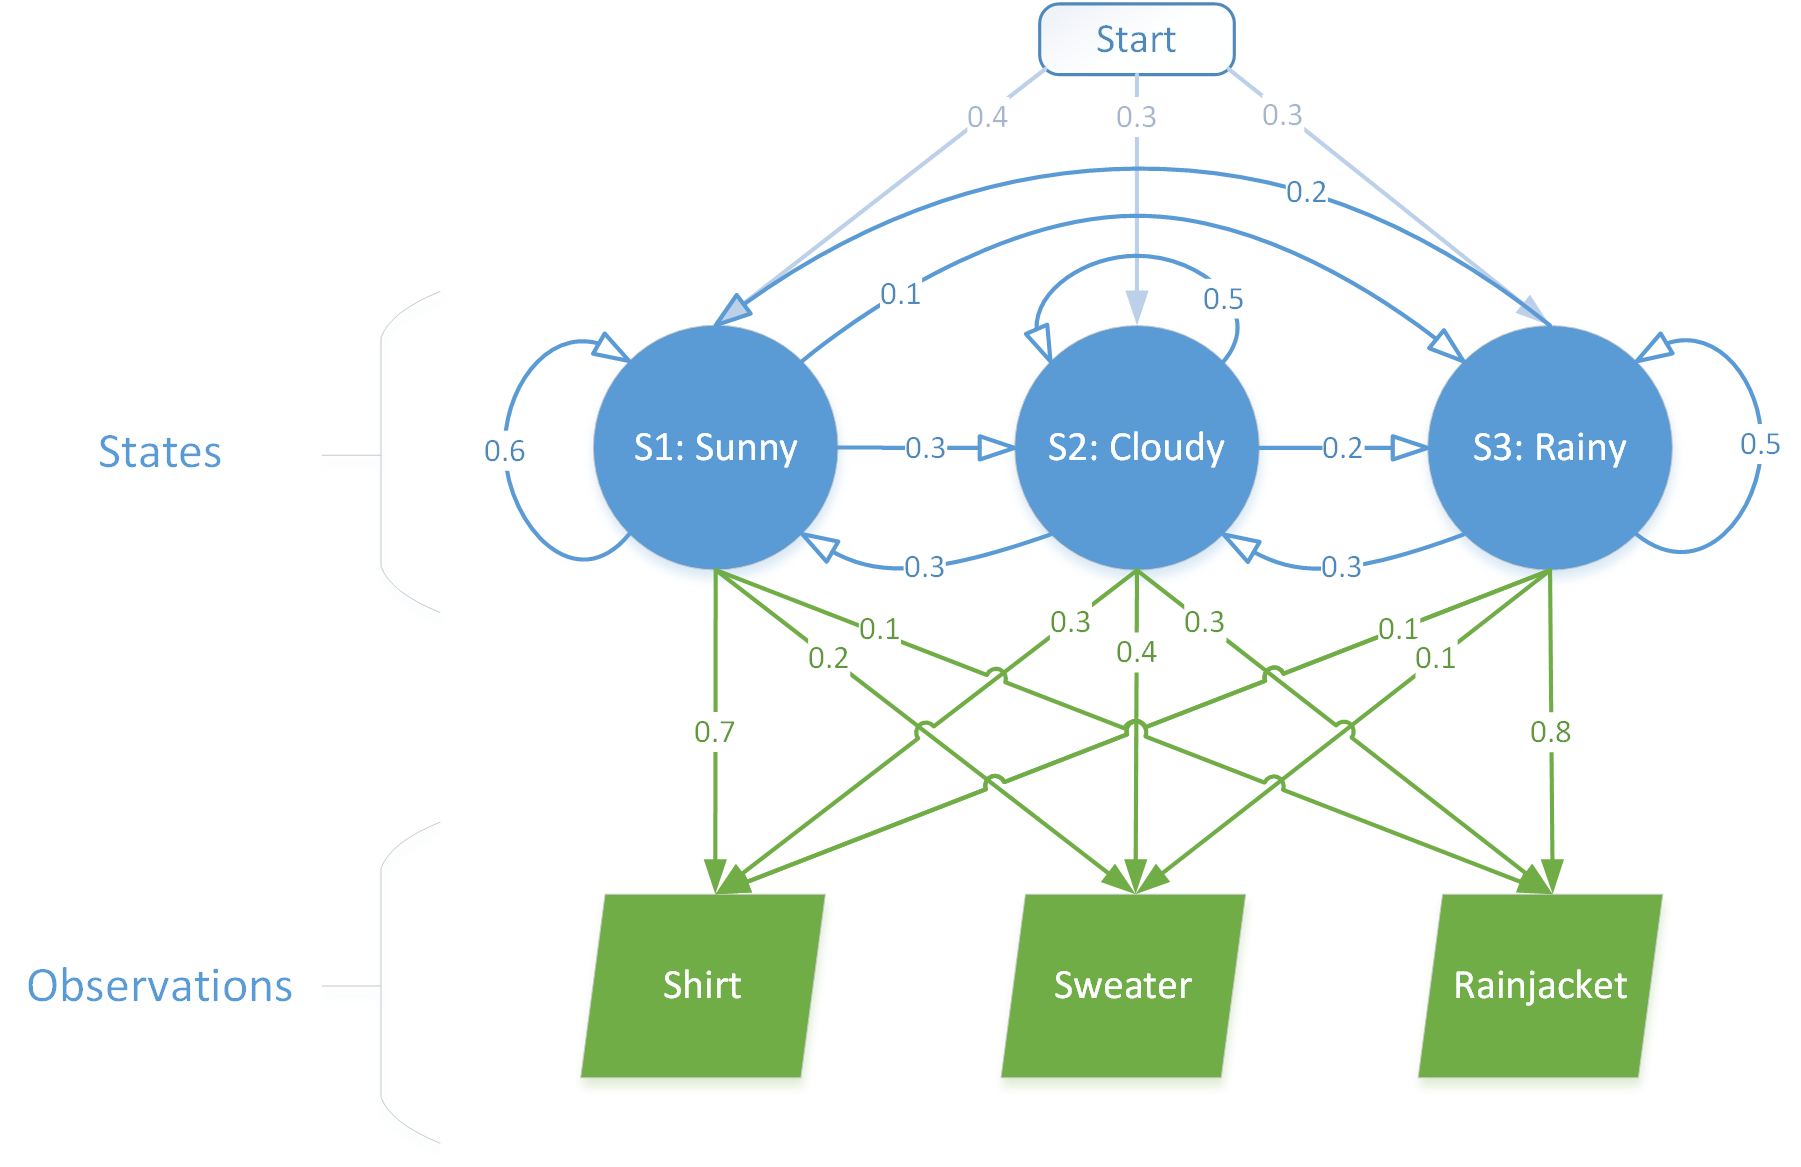
\includegraphics[width=0.82\linewidth]{../modelDevelopmentFlowcharts/HMMDiagram.png}
	\caption{Markov Model}
	\label{fig:HMM}
\end{figure}

The appropriately named Hidden Markov Models (HMM) are simply Markov Models where the underlying states are hidden - i.e. cannot directly be observable \cite{Jurafsky2017,Bobick2015a,Gagniuc2017,OConnell2011,Rabiner1989}. Specifically, while we may know the number of states in the model, the transition probabilities of the model, we don't know the exact state the system is in or the sequence of states it has been through \cite{Jurafsky2017,Bobick2015a,Gagniuc2017,OConnell2011,Rabiner1989}. However, given the observation probabilities it is possible for us to try and infer the current state of the Model, including the sequence of states that a particular Markov Model went through \cite{Jurafsky2017,Bobick2015a,Gagniuc2017,OConnell2011,Rabiner1989,Mailund2014}. This is because Hidden Markov Models, as with Markov Models, operate under the Markovian assumption: they assume that the process they model adhere to the Markovian property \cite{Rabiner1989,Jurafsky2017,Bobick2015,Bobick2015a}. However, it has been found that Hidden Markov Model are able in certain cases to fairly successfully model processes that violate this Markovian assumption such as speech recognition and gesture recognition \cite{Altman2007,Jelinek,Rabiner1989}. Part of contributions of this study will be to determine if Hidden Markov Models are suitable for modelling patient activity and heart rate data both of which likely violate the Markovian assumption 'demanded' of Hidden Markov Models.

\paragraph{Semi-Markov Model}

The violation of the pure Markovian assumption leads us to a variation on Hidden Markov Models: Hidden Semi-Markov Models (HSMM) \cite{OConnell2011}. HSMMs are HMMs that formally relax the 'Markovian' assumption of the model by permitting the model to specifically retain the memory of how long it has been in a certain state (typically in order to force the model to not exist in a state for more than a desired time) \cite{OConnell2011}. As such, HSMMs require that an additional set of parameters be defined: the sojourn distribution of each state \cite{OConnell2011}. That is, the distribution of expected mean waiting times in each given state. These waiting times can follow any distribution desired - normal, geometric, gamma, etc. - or appropriate for the problem at hand \cite{OConnell2011}. 

In our case, since it is probably unreasonable to assume that there no some time-dependence in state changes due to the dynamic nature of human exercise and activity (e.g. people who are performing high-intensity activity are less likely to continue as time goes by since they get tired) we propose also training equivalent multivariate hidden semi-Markov models for each of the target risk groups to explore the effect of relaxing the Markovian assumption (or time-independence) of pure Markov models if the regular pure Markov models prove to be unsuitable for our study. 

\paragraph{Parameters Required for Hidden Markov \& Semi-Markov Models}

To summarize, the complete set of parameters that must be determined for a Hidden Markov Model are as follows:
\begin{enumerate}
	\item the number of states in the model
	\item the starting probabilities
	\item the transition probabilities
	\item the (observation) emission probabilities
\end{enumerate}
For Hidden Semi-Markov Models, we add the additional parameter of the individual state sojourn distributions.

\paragraph{Determining Markov Model Parameters}

Determining the single best or most optimal Hidden Markov Model parametrization for given data stream is unfortunately, an intractable problem \cite{Rabiner1989,Gagniuc2017,Jurafsky2017}. That being said, there is a known algorithm for efficiently computing the most likely locally optimal parametrization, the maximum likelihood estimation, for a stream. Generally speaking the specific sub-class of algorithms used to solve this problem in the markov model space are known as expectation-maximization (EM) algorithm \cite{Rabiner1989,Gagniuc2017,Jurafsky2017}. One of the most common EM algorithm implementations used for Hidden Markov Model training is the Baum-Welch algorithm \cite{Rabiner1989,Gagniuc2017,User347902016,Jurafsky2017}. Another common algorithm used to approximate EM is the Viterbi \textit{training} algorithm (N.B. not the Viterbi algorithm) which can yield less accurate models than the Baum-Welch algorithm but is usually much less computationally intensive \cite{Rodriguez2003,User347902016}. We eschew further discussion of the implementation details of either of these algorithms since the availability of pre-programmed libraries implementing these algorithms makes it unnecessary for any given arbitrary reader to have the in-depth knowledge required to implement the algorithms and because there are many excellent sources available that explain the fine details of algorithm probably much better than this author could \cite{Rabiner1989,Rodriguez2003,Gagniuc2017,Jurafsky2017}. In any case none of these algorithms is able to determine all of the parameters by itself. Some of the parameters must be provided as 'initial conditions' for the algorithm to execute. Typically these are the emission probabilities, the starting probabilities, the sojourn distributions (and sometimes even initial transition probabilities). Depending on the library used it may try to make an educated guess for starting points or leave the 'initial conditions' to be specified solely by the author. It is possible (and encouraged) to try various combinations of parameters to determine the most effective set - in fact more fully featured software libraries will also sometimes offer to do this automatically, although it is ultimately up to the researcher to determine appropriate 'initial conditions.'

In our case we use the 'mhsmm' package for the R software platform \cite{OConnell2011,OConnell2017} which requires the user to provide the number of desired states, the emission probabilities (which are assumed to remain fixed) as well as an initial starting point for the state probabilities and transition probabilities, which the algorithm then adjusts as it searches for a local optimum.

\paragraph{Proposed Initial Markov Model Parameters}

For this study we anticipate to start with the following initial conditions:
\begin{enumerate}
	\item \textbf{States}: We begin with 3 initial states and then sweep from 3 to 6-8 states depending on the available computational power. The computational power limit is important since computational complexity for training Hidden Markov Models increases to the square of the number of states as a result of the states being interconnected. That is, with 3 states there are 9 possible transitions between states which must be solved. Doubling the number of states to 6 causes a quadrupling of the number of possible transitions to 36. At 8 states there are 64 possible transitions, almost double that of the 6 state case which may make such an HMM too unwieldly for us to train given available resources.
	\item \textbf{Starting State Probabilities}: We set a probability of 1 (i.e. 100\% likelihood) for one of the states and 0 for all the others. We anticipate that this will be a good starting point based on initial exploration of the data that seemed to indicate that patients spend most of their time in a non-active state. In other words, at any given moment of we were to look at the time stream it is most likely that a patient will be in the non-active state as opposed to any other state so we reflect this in the starting probabilities.
	\item \textbf{Transition Probabilities}: Given a lack of evidence to the contrary we make the simple assumption that the transition probabilities are uniform and so set each to be the reciprocal of the number of state transitions. In other words, if the we let $n_s$ be the number of possible states, and $n_t$ be the number of possible state transitions, the initial transition probabilities $P_t$ are each $P_t = \frac{1}{{n_s}^2} = \frac{1}{n_t}$.
	\item \textbf{Emission Probabilities}: Based on previous analysis of the data the minute-by-minute step counts appear to be approximately gamma distributed with peaks (or sub-peaks) clusters. We therefore propose setting the emission probabilities to be gamma distributed such that the distributions center around prominent peaks visually identified from the data: e.g. 20 steps/min, 80 steps/min, 100 steps/min for a 3 state HMM. For heart rate emission probabilities we similarly propose using normal distributions initially centred around the traditional heart rate zones which for a normal healthy human are defined as follows \cite{FitbitInc.2017}:
	\begin{enumerate}
		\item resting: 60 bpm
		\item above resting but \textless50\% of max, slightly elevated: 89 bpm
		\item 50 to 69\% of max, low intensity exercise: 110 bpm
		\item 70 to 84\% of max, medium intensity exercise: 135 bpm
		\item 85\% to 100\% of max, high intensity exercise: 152 bpm
		\item $\geq$100\% of max, maximum intensity exercise: 220 bpm - age
	\end{enumerate}
	\item \textbf{Sojourn Distributions}: For exploration of Hidden semi-Markov Models the propose using an identical gamma distribution for each state to model the mean waiting time. The gamma distributions would be centered around a certain period of time, sweeping that period of time in 1hr intervals from 1 to 12 hrs, under the assumption that our patients person, despite their condition, will likely have to get up (or attempt to get up - thereby registering even momentary activity) once a day to attend to essential needs.
\end{enumerate}

Now that we have reviewed the essentials of Markov Models and how to compute the parameters of a Hidden Markov Model in general (including the proposed initial parametrizations of each of the models) we proceed to discuss how we propose to use Hidden Markov models to classify patients.

\paragraph{Classification}

A previously mentioned to perform the classification we propose creating and train multivariate Hidden Markov Models for each of the target risk groups (NYHA class II, III, IV). We can collect the Hidden Markov Models that were generated into a sets with a Hidden Markov Model for each risk group, i.e. for a binary classifier the sets would consist of 1 HMM trained using NYHA class II patients, and 1 using NYHA class III patients. By extension for the 3 class multi-class classifier the sets would additional contain a HMM trained using NYHA class IV patients. Classification can then be performed by evaluating the likelyhood that a given (unclassified) patient's sequence (i.e. activity, heart rate data stream) was generated from each of the corresponding HMMs in a set - the evaluation of which can be performed using either the forward or backward algorithm detailed in any of these referenced works, and whose functionality is included in most HMM programming libraries \cite{Jurafsky2017,Bobick2015a,Gagniuc2017,OConnell2011,Rabiner1989}. The predicted classification of the patient would then correspond to the class of the model with the highest likelihood of having 'generated' that data stream. This process is detailed graphically in Figure \ref{fig:C2}. In an ideal system we would select the single set of Hidden Markov Models that would be able to best classify patients into their appropriate class - how we go about selecting this set is detailed later in this section as part of the Hidden Markov Model training. In general though, and in particular within the context of a larger system in which patients might be stratified by other variables, such as sex or the use of a certain medications (e.g. beta-blockers), one could feasible also train an ideal Hidden Markov Model set for each patient sub-group or stratification. This process by which this is done for a group of patients, collected together as the \textit{Data} block is detailed graphically in Figure \ref{fig:C0C1}. The output of this process can be constructed as a table where each patient is listed along with it's corresponding predicted class - a \textit{Patient Class Table}.

\landscapeFigure{1cm}{C2: Classifier - Classify Using Model Set}{../modelDevelopmentFlowcharts/C2-Classifier_Classify_Using_Model_Set.png}{fig:C2}

\landscapeFigure{1cm}{C0\&C1 Classifier - Generalized System}{../modelDevelopmentFlowcharts/C0&C1-Classifier_Overview.png}{fig:C0C1}


\paragraph{Training: Preparing \& Preprocessing of Data}

Having outlined how the proposed NYHA classifer is supposed to work we turn to the task of training a system, that is, determining the ideal Hidden Markov Model set for a provided set of input patients. As a first step to this training however it is important that we first preprocess and clean the \textit{raw data} that we will use as input. The preprocessing procedure is outlined in Figure \ref{fig:P0}. First the raw data is passed through an \textit{automated cleaner} which is an script that 'cleans' and standardizes the data before use, including removing or filling in missing variables as required, standardizing keywords so that they all follow the same format (e.g. NYHA Class II is cleaned and converted so that it is always internally represented as 'II' instead of 'ii','2','two' or any other variants) or removing characters, data elements or otherwise that are not needed or might even cause problems with any other downstream processing elements. This automated cleaner is updated as required on each pass (by the author) to include any common items that have been detected during manual cleaning and verification of the data so that the system can more easily be transferred to a live clinical environment and to improve the ability of the \textit{automated cleaner} to completely clean the data. After passing through the \textit{automated cleaner} and before \textit{Manual Cleaning and Verification} the data is passed through a preprocessing and formatting step where the data is converted from the raw input data type (for example tab-deliminated string) into a format more amenable for the processing environment (for example an R dataframe, vector or matrix). As previous mentioned, after this step the data is manually verified to catch any obvious errors. The output of this last verification process is the 'Processed Data'.

Due to the particular circumstances of our study, namely that the data set collected is too small to perform practical machine learning which requires a large amount of data this \textit{processed data} undergoes another transformation before it is used to train our machine classifier. This is the microsimulation step. Microsimulation is useful in the case where a particular machine learning algorithm needs to see a minimum 'critical mass' of data in order to be able to begin to successfully classify inputs. Specifically microsimulation allows us to generate an arbitrary amount of simulated 'fake' data from an original dataset based on pre-identified statistical properties of the original dataset (with a little added noise for variance). The idea is that since this simulated data is (statistically) representative of the original data the machine learning algorithm will pick up on the same traits as it would have from an original larger dataset but without requiring that larger dataset in the first place. There are of course limitations to the inferences we can make on the classification accuracy of a machine learning model trained using microsimulated data, but it is a useful tool for demonstrating proof of concept. In Figure \ref{fig:P0} microsimulation is shown as being performed in two parts, first the statistical properties of the \textit{processed data} analysed and the results of this analysis are then used to \textit{microsimulate} (i.e. generate) the \textit{$\mu$Simulated Data For Training}. This \textit{$\mu$Simulated Data For Training} forms the dataset used for the rest of the development of the models. Although for the purposes of this explanation we do not stratify the patients, the process of stratification, if required, would be performed after generating the processed data and before performing the microsimulation (including both the analysis of statistical properties and the \textit{microsimluate} steps). Stratifying patients at this point allows us to generate a corresponding dataset of \textit{$\mu$Simulated Data For Training} for each patient strata which we can separately feed as the input for the rest of the training process until we have generated the corresponding Hidden Markov Model set for each of the strata.

\landscapeFigure{1cm}{P0: Preprocessing Data}{../modelDevelopmentFlowcharts/P0-Preprocessing_Data.png}{fig:P0}

\paragraph{Training: Model Selection}

After converting the raw data into clean and usable format we can proceed to the actually generation, training and selection of our candidate Hidden Markov Models. Overall the general process, which is shown in Figure \ref{fig:T0} is as follows:
\begin{enumerate}
	\item Generate potential models, which we store as a \textit{Potential Model List}. 
	\item Apply each generated candidate model to each patient in the \textit{$\mu$Simulated Data For Training} provided as input. We do this to evaluate the probability that each candidate model generated the corresponding patient data stream. We keep these probabilities in a table which links each model to the probability it generates for each patient; this is the \textit{Model-\textgreater Patient Probability Table}.
	\item Based on the generated \textit{Model-\textgreater Patient Probability Table} and the true class which we can extract from the \textit{$\mu$Simulated Data For Training} provided as input we can evaluate determine the best model set of the candidate sets generated. 
	\item Lastly we return the best model identified in the previous step.
\end{enumerate}

\paragraph{Training: Model Generation}

The process of generating multiple models can be divided, at least logically, into two seperate parts. The first is that of generating a models for each of the classes. The second involves generating different models within each class group using different initial HMM parameters with the goal of trying to find a parametrization that is closest to the representing the true underlying 'model' for that class group (i.e. the globally optimal parametrization as opposed to simply a locally optimal parametrization). Both of these are faily simple and the combined process is detailed in Figure \ref{fig:T1}. 

The first part, generation for each class can be accomplished by simply selecting all the patients that belong to given class from the input \textit{$\mu$Simulated Data For Training} and using these as the training data for the model training function \textit{hmm.fit} of our HMM library for R: 'mhsmm'. This training function outputs a potential model which we can add to our \textit{Potential Model List} which we will return at the end of the generation process. 

The second part, generating different parametrizations, is combined as part of the class by class generation and simply involves updating the initial parameters that form the second half of the required input for the \textit{hmm.fit} training function until we have swept through all the desired parameter variations.

\paragraph{Training: Extracting the Ideal Model Set}

The process of extracting the ideal, or single best model set from the generated \textit{Potential Model List} is also fairly simple and is detailed in Figure \ref{fig:T2}. We can simply iterate through every possible model set, i.e. each possible combination of NYHA class II, III and IV models (for the 3 class multi-class classifier) and evaluate the performance score of each model set by comparing the \textit{True Classes for Patients} against the \textit{Predicted Classes for Patients} generated by the classifier resulting from that set of HMMs (recall Figure \ref{fig:C2}). We can store these scores as a \textit{Model Set-\textgreater Score Table} for future review or as detailed in Figure \ref{fig:T0} simply return the single best model combination. The process in Figure \ref{fig:T2} outlines the storage method since it is most useful for a researcher, who may wish to review the score results to perform additional analyses on the performance scores.

\paragraph{Training: Model Evaluation}

The process by which the performance scores of each model can be evaluated is visually detailed in Figure \ref{fig:T3}. This particular process however is described in detail in section \ref{sec:classperformance} of this document.

\landscapeFigure{1cm}{T0: Training - Model Selection}{../modelDevelopmentFlowcharts/T0-Training_Model_Selection.png}{fig:T0}

\landscapeFigure{1cm}{T1: Training - Potential Model Generation}{../modelDevelopmentFlowcharts/T1-Training_Potential_Model_Generation.png}{fig:T1}

\landscapeFigure{1cm}{T2: Training - Extraction/Selection of Ideal Model Set}{../modelDevelopmentFlowcharts/T2-Training_Extract_Ideal_Model_Set.png}{fig:T2}

\landscapeFigure{1cm}{T3: Training - Model Evaluation}{../modelDevelopmentFlowcharts/T3-Training_Model_Evaluation.png}{fig:T3}

------------

\paragraph{Summary}

In summary, we reviewed the basics of Markov Models including variations on the such models where the underlying assumptions are relaxed. We also outlined the method by which we develop a binary or 3 class multi-class classifier that uses sets of multivariate Hidden Markov Models to classify patients into their corresponding NYHA class within the subset of classes supported by the classifier. We do this by generating several possible sets of Hidden Markov Models for each corresponding class and selecting the combination of models amongst those generated that produce the most performant classifier according to the performance metrics outlined in the next section (section \ref{sec:classperformance}) although we provide a brief visual summary of the evaluation procedure.

\subsubsection{Classifier (Model) Performance Assessment} \label{sec:classperformance}

\paragraph{Confusion Matrix}

After development of an classification algorithm it will be important to assess how well the classifier is able to correctly assess patient NYHA class. Since performance evaluation measures differ for binary and multi-class classifiers this section discuss both. Measures of classification accuracy for a classification test or algorithm (regardless of the number of supported classes) can be reported in a confusion matrix, an example of which is shown below \cite{Sayad,MedCalc2017,Davis2006,Flach2004}.

\renewcommand{\arraystretch}{1.5}
% 3 Class Confusion Matrix
%  https://tex.stackexchange.com/a/20295
\begin{center}
	\begin{tabular}{l|l|c|c|c|c}
		\multicolumn{2}{c}{}&\multicolumn{3}{c}{Clinical Classification}&\\
		\cline{3-5}
		\multicolumn{2}{c|}{}&II&III&IV&\multicolumn{1}{c}{Predictive Value:}\\
		\cline{2-5}
		\multirow{5}{0.8cm}{\rotatebox{90}{\parbox{0.8cm}{\centering Algorithm \\ Classification}}} % adjust this spacing to shift left/right
		& II & $a$ & $b$ & $c$ & $\frac{a}{a+b+c}$\\
		\cline{2-5}
		& III & $d$ & $e$ & $f$ & $\frac{e}{d+e+f}$\\
		\cline{2-5}
		& IV & $g$ & $h$ & $i$ & $\frac{i}{g+h+i}$\\
		\cline{2-6}
		\multicolumn{2}{c}{Sensitivity:} & \multicolumn{1}{c}{$\frac{a}{a+d+g}$} & \multicolumn{1}{c}{$\frac{e}{b+e+h}$} & \multicolumn{1}{c}{$\frac{i}{c+f+i}$} & \multicolumn{1}{|c}{Accuracy:}\\
		\multicolumn{2}{c}{Specificity:} & \multicolumn{1}{c}{$\frac{e+f+h+i}{b+c+e+f+h+i}$} & \multicolumn{1}{c}{$\frac{d+f+g+i}{a+c+d+f+g+i}$} & \multicolumn{1}{c}{$\frac{d+e+g+h}{a+b+d+e+g+h}$} & \multicolumn{1}{|c}{$N=\frac{a+e+i}{\sum_{}^{}all cells}$}\\
	\end{tabular}
\end{center}

%% 2 Class Confusion Matrix
%\begin{tabular}{l|l|c|c|c}
%	\multicolumn{2}{c}{}&\multicolumn{2}{c}{Clinical Classification}&\\
%	\cline{3-4}
%	\multicolumn{2}{c|}{}&I&II&\multicolumn{1}{c}{Predictive Value:}\\
%	\cline{2-4}
%	\multirow{2}{2cm}{Algorithm Classification} % adjust this spacing to shift left/right
%	& I & $a$ & $b$ & $\frac{a}{a+b}$\\
%	\cline{2-4}
%	& II & $c$ & $d$ & $\frac{c}{c+d}$\\
%	\cline{2-5}
%	\multicolumn{1}{c}{} & \multicolumn{1}{c}{} & \multicolumn{1}{c}{Sensitivity:} & \multicolumn{1}{c}{Specificity:} & \multicolumn{1}{|c}{Accuracy:}\\
%	\multicolumn{1}{c}{} & \multicolumn{1}{c}{} & \multicolumn{1}{c}{$\frac{a}{a+c}$} & \multicolumn{1}{c}{$\frac{d}{b+d}$} & \multicolumn{1}{c}{$\frac{a+d}{a+b+c+d}$}\\
%\end{tabular}
%\linebreak

\paragraph{Standard Performance Measures}

From the cells of a confusion matrix we can, amongst other measures, determine the:
\begin{enumerate}[label=\alph*)]
	\item \textit{sensitivity}, \textit{recall}, or \textit{true positive rate} of a test: the proportion of patients correctly identified as belonging to the particular test class e.g. class II \cite{Flach2004,MedCalc2017,Gung2013,Sokolova2009,Forman2010,VanAsch2013}. Phrased mathematically, letting $x_c$ represent those patients belonging to a particular class $c$ (e.g. class II) from the set of all classes $C$ and $\hat{x_c}$ represent those patients predicted by the test as belonging to this particular class then the sensitivity is $P(\hat{x_c}|x_c)$. In other, words sensitivity measures how reliably the test identifies patients belonging to a particular class by labelling them with that class. 
	\item \textit{specificity}, or \textit{true negative rate} of a test: the proportion of patients correctly identified as not belonging to the particular test class e.g. not class II \cite{Flach2004,MedCalc2017,Gung2013,Sokolova2009,Forman2010,VanAsch2013}. Phrased mathematically, letting $!x_c$ represent those patients not belonging to a particular class $c$ (e.g. not class II) and $\hat{!x_c}$ represent those patients predicted by the test as not belonging to class $c$ then the sensitivity is $P(\hat{!x_c}|!x_c)$. In other words, specificity measures how reliably the test identifies patients not belonging to a given class by labelling with a class other than that given class.
	\item \textit{fall-out}, or \textit{false positive rate} of a test: the proportion of patients positively identified by the test as belonging to a particular class but actually belonging to a different test class e.g. identified as class II but actually class I \cite{Flach2004,MedCalc2017,Sokolova2009,Forman2010,VanAsch2013}. Phrased mathematically using the same definitions as for the previous measures then the false positive rate is $P(\hat{x_c}|!x_c) = 1 - \textit{specificity}$. In other words, the false positive rate identifies how over-eager the test is at labelling patients as belonging to a particular class in an effort to not miss patients that actually belong to that class - it is the 'fall-out' or 'collateral damage' in the 'affirmative' labelling.
	\item \textit{precision} or \textit{positive predictive value} of a test: the proportion of patients correctly classified as belonging to a particular test class amongst all those identified by the test as belonging to that class \cite{Flach2004,Gung2013,Sokolova2009,Forman2010,VanAsch2013}. Phrased mathematically using the same definitions as for the previous measures then the positive predictive value is $P(x_c|\hat{x_c})$. In other words, the positive predictive value measures how likely a patient is, for each given class, to actually belong the class it has been labelled as.
	\item \textit{accuracy} of a test: the proportion of patients correctly classified by the test into their true class \cite{Flach2004,MedCalc2017,Sokolova2009,Forman2010,VanAsch2013}. Phrased mathematically using the same definitions as for the previous measures the accuracy of the test is $\bigcup P(\hat{x_c} = x_c)$ for all $c\in C$ which in the case of mutually exclusive classes simplifies to $\sum\limits_{c\in C}P(\hat{x_c} = x_c)$. In other words, the accuracy measures how well a test correctly classifies patients into their respective classes. Unfortunately, the way accuracy is calculated makes it highly sensitive to the underlying base rate of occurrence of each of the classes, namely it preferentially weighs classes that occur more frequently in the underlying population often limiting it's usefulness as a summary metric.
	\item \textit{F score}, \textit{$F_1$ score}, or \textit{F-measure} of a test: an alternative to accuracy that is less sensitive to the underlying base rate of occurrence for each of the classes. It is the harmonic mean of \textit{precision} and \textit{recall} for that class \cite{Flach2004,MedCalc2017,Sokolova2009,Forman2010,VanAsch2013}. Phrased mathematically using the same definitions as for the previous measures the F score of the test is: \newline$F_1 = 2*(\frac{1}{\textit{recall}} + \frac{1}{\textit{precision}})^{-1}$
\end{enumerate}

\paragraph{Receiver Operating Characteristic \& Area Under Curve}

To aid in comparing performance, many of the above test measures can be visualized in various ways. One of the most useful is the Receiver Operating Characteristic (ROC) curve which shows the trade off between the \textit{sensitivity} and \textit{fall-out} of a test \cite{Davis2006,Sayad,Fieldsend2005,Flach2004,MedCalc2017,Gung2013}. We can generate the ROC curve for each risk group by plotting the corresponding risk group \textit{false positive rate} vs \textit{true positive rate}. Alternatively, we can also generate a precision-recall (PR) plot to better understand the trade-off relationship between the precision vs recall for each group \cite{Davis2006,Flach2004,MedCalc2017,Gung2013}. While both of these plots are very useful for visual comparison of the performance trade-offs between different algorithms (or even different formulations or parametrizations of the same algorithm) it is often very useful to be able to distil these visual plots into a single performance metric to make a final determination on algorithm performance. This is especially true in the case where an algorithm designer would like to automate the search for the optimal algorithm (parametrization or formulation).

Both the ROC and precision-recall plots are easily interpretable and can be summarized by measuring the areas under each of the ROC and precision-recall curves (ROC AUC and precision-recall AUC respectively) \cite{Davis2006,Flach2004,MedCalc2017,Sayad}. Plots with an AUC value closer to 1 represent better overall classifiers (AUC values lower than 0.5 indicate performance that is worse than random classification). AUC values are convenient for comparing multiple ROC or precision-recall plots but are generally not recommended as the sole decision criteria \cite{Davis2006,Flach2004,MedCalc2017,Sayad}. This is simply because a unidimensional metric inevitably obfuscates the underlying curve (recall the moral of Anscombe's quartet) \cite{Anscombe1973}.

\paragraph{Binary Classifier Performance Evaluation}

In the case of a binary (mutually exclusive two-class) classifier (e.g. where the decision must be made to classify a patient into NYHA class II or III only), which can be summarized using a single ROC or precision-recall (PR) curve (since, by symmetry, improving the classification of one class reduces the misclassification of the second and vice versa), selecting either the ROC AUC or precision-recall AUC is natural, expedient and generally very effective \cite{Davis2006,Flach2004,MedCalc2017,Sayad}. However the selection of ROC AUC over precision-recall (PR) AUC depends on the underlying class balance of the dataset. David et al.\@ proved a 'surprising theorem that a curve dominates in ROC space if and only if it dominates in PR space' but 'that an algorithm that optimizes the area under the ROC curve is not guaranteed to optimize the area under the PR curve' \cite{Davis2006}. Precision-recall curves, and by extension the PR AUC, are more appropriate for use in datasets with highly skewed class distributions (e.g. a prevalent negative class with few positive class - very common in the field of information retrieval) \cite{Davis2006,Flach2004,Sokolova2009}. Precision-recall curves however are more computationally complicated to solve although several packages exist for the R programming language (amongst others) to calculate PR AUC, ROC AUC and all the various metrics discussed thus far \cite{Robin2017,Yan2016}.

\paragraph{Multi-class Classifier Performance Evaluation}

In the case of multi-class classifiers (e.g. where the decision presented is to classify a patient into any of the four classes, or even just three of the four classes: e.g. II-IV) the situation is more complicated. Multi-class classifiers cannot be summarized using a single ROC or precision-recall curve in the same way as binary classifiers \cite{Sokolova2009,Flach2004,Fieldsend2005,Hand2001a,Hyndman2010,Kautz2017}. There have been attempts by researchers to develop an equivalent AUC metric by expressing it in an 'equivalent probabilistic form' \cite{Hand2001a}, or by plotting multi-dimensional ROC or precision-recall surfaces - although this metric is more accurately termed the volume-under-the-curve (VUC) for the 3 class case, hyper-volume-under-the-curve (hVUC) for the 4 class case, and so on \cite{Fieldsend2005}. None of these metrics however has gained widespread acceptance. The most accepted approach however appears to be to completely forgo calculation of the AUC in the first place and instead perform a micro- or macro-average of an underlying performance measure (such specificity) \cite{Flach2004,Sokolova2009,Hyndman2010}. 

\paragraph{Macro- and Micro-Averaging}

The macro-average of a measure, is calculated in the same way as one might compute the 'classical' mean of a the measure by simply taking the mean of the measure output values. The micro-average however involves instead first taking the mean of the inputs to the measure computation function and using those input mean values to calculate a single measure output value \cite{VanAsch2013}. The difference is sometimes clearer and more obvious when expressed mathematically.

Given a set of $k$ classes $C = {c_1,c_2,...c_k}$ and a binary performance measure $B(m_{1,c},m_{2,c},...,m_{n,c})$ that can be calculated for a given class $c$ (and for each class $c$) based on a values in the confusion matrix $m_{1,c}$ to $m_{1,n}$ for that class (which in our case would be the main confusion metric measures: true positives \& negatives and false positives \& negatives) then the macro-average is for performance measure $B$ is calculated as \cite{VanAsch2013,Forman2010,Tsoumakas2009}:

\begin{equation}
B_{macro} = \frac{1}{k}\sum\limits_{j=1}^{k}B(m_{1,j},m_{2,j},...,m_{n,j})
\end{equation}

\noindent In comparison the micro-average is calculated as \cite{VanAsch2013,Forman2010,Tsoumakas2009}:
\begin{equation}
B_{micro} = B(\sum\limits_{j=1}^{k}m_{1,j},\sum\limits_{j=1}^{k}m_{2,j},...,\sum\limits_{j=1}^{k}m_{n,j})
\end{equation}

\paragraph{Effects of Class Imbalance}

Unfortunately, it is still an open question as to whether micro-averaging or macro-averaging produces more reliable results. Van Asch quoting a paper by Sebastiani outlines the state of the debate in the early 2000's \cite{VanAsch2013}:
\blockquote{There is no complete agreement among authors on which is  better. Some believe that  “micro-averaged performance is somewhat  misleading (...) because more frequent topics are weighted heavier in the average” [Wiener et	al. 1995, page 327] and thus favour macro-averaging.  Others (actually, the majority of researchers) believe that topics should indeed count proportionally to their frequence, and thus lean towards micro-averaging.\cite{Sebastiani2002}} The choice is sometimes performance measure dependent; Forman et al.\@, based on series of simulations they performed, advanced the majority position that micro-averaging should be the preferred method for calculating the F score (a common alternative to accuracy in the information retrieval domain) since it is more unbiased in the common case where class imbalance exist in those datasets, especially where that class imbalance is large or the classifier is inaccurate in the first place \cite{Forman2010}. A decade and a half later, the issue, at least in practice, appears to still not be settled. A quick review of recent literature shows that researchers appear to prefer to simply use and report both the micro- and macro-averaged results for their metrics (usually precision, recall, accuracy and F score) \cite{Rehman2017,Du2017,Kayaalp2017,Wang2014}. Some have even eschewed micro- and macro-averaging in favor of developing new metrics, such as the Multiclass Performance Score (MPS), designed specifically for use with multi class classifiers \cite{Kautz2017}. In keeping with common practice we plan to report on the micro- and macro-averaged precision, recall, accuracy and F score of our algorithm. But, in our case, given our intent to integrate our classification algorithm into a larger clinical decision support application at the Heart Failure Clinic we do not have the freedom of waffling between all of these measures but rather must make a determination of which single measure is most appropriate for the evaluation of our candidate algorithms for optimization. To do this we return to the basics.

The fundamental difference between macro- and micro-averaging is how the weighting is distributed. In macro-averaging equal weight is given to each class. In micro-averaging equal weight is given to each individual patient classification decision. To Forman et al.'s point, it's not that micro-averaging is more unbiased so much as it's particular bias was more suitable given the field of application considered by Forman et al. (namely document retrieval where giving adequate weighting to less frequently occurring individual results - typically the documents to be retrieved - is more preferable). In a sense, every measure is biased - the question is simply which bias is more helpful for the application in question. 

In our case we also expect to have an imbalance of persons in each class for various reasons: 
\begin{enumerate}[label=\alph*)]
	\item sicker patients (closer to class IV) are more likely to die and therefore those classes are likely to be more under represented,
	\item the UHN Heart Failure clinic typically sees more advanced cases of Heart Failure and is less likely to see patients in the lowest class (class I) making this class more likely to be under represented\footnote{which again, is also why although the general approach proposed is easily extensible to this class, NYHA class I patients are generally disregarded in our study},
	\item based on our previous experience with the Medly tele-monitoring platform, class IV patients are less likely to be prescribed the platform as a clinical intervention (and thus be eligible for the study) since physicians perceive them to be less likely to benefit from the intervention. As a result, this class is again more likely to be under represented.
\end{enumerate}

Of course we will need to examine the final recruitment cohort to confirm that our expectations do indeed turn out. Have established that "microaveraged results are ... really a measure of effectiveness on large classes in a test collection. To get a sense of effectiveness on small classes, [one] should compute macroaveraged results" \cite{Manning2009}. This would indicate that the use of macro-averaging will provide the most suitable bias for our particular situation since, as discussed, NYHA class IV is likely to be under represented in our population. Since macro-averaging will treat every class considered with equal weighting optimizing our algorithm using a macro-averaged metric is more likely to ensure that classification performance of a smaller NYHA class IV will be treated with the same priority as any other class. Optimizing using micro-averaging would instead preferentially weigh improvements (or decreases) in algorithm performance that largely affect those classes whose patients are more represented in the dataset (NYHA class II or III) which we suggest is undesirable.

Of course we do note that the use of microsimulation allows us to compensate for any significant imbalances in our development dataset by allowing us to simulate (i.e. generate) a balanced dataset should we so choose.  The issue of micro- vs macro-simulation therefore is perhaps less critical for this particular study as it may be for future (external) validation studies.

\paragraph{Misclassification Costs}

So putting aside the issue of micro- and macro-averaging for a moment. Thus far we have entirely avoided the issue of misclassification cost. For binary classification problems misclassification cost is generally glossed over since there is only a single cost for incorrect classification. This cost can be taken into account after computation of performance measures. However, in certain multi class classification problems (such as this one) certain types of misclassification can been deemed to be more costly than others and so there is not necessarily a single cost for misclassification. In our case: misclassification of a class II patient into class IV is a more severe error, and thereby most costly error, than misclassification of a class II patient into class III. It is a relatively easy task to design an algorithm to account for this and so the difficulty here mostly revolves around how to quantify the exact costs of different degrees of misclassification (costs which also could very well change over time) \cite{Kautz2017}. This challenge is rendered even more difficult since classification of patients into NYHA class, as already mentioned, is already an unreliable art \cite{Carroll2014,Goldman1981a,Raphael2007a,Kubo2004}. And where there is already a relative paucity of published research regarding the reliability of NYHA classification by physicians there is complete drought when it comes to attempts to quantify the real costs of misclassification. Fortunately selecting an incorrect misclassification cost in this context will not actually reduce the accuracy of a selected output algorithm. Instead it would direct the optimization algorithm to search for a suboptimal algorithm, not that any optimization algorithm even guarantees that it has found the single most (i.e. globally) optimal algorithm in the first place \cite{Segaran2007}. Given the aforementioned consideration and the lack of readily available data documenting concrete misclassification costs we propose the following as a reasonable selection of costs to use as a starting point in this study. Of course, we invite the interested reader to improve on our approach.

\paragraph{Derivation of a Performance Metric that accounts for misclassification costs and class imbalance}

Recall that \textit{true positive rate} (\textit{sensitivity}/\textit{recall}) measures the proportion of patients correctly identified as belonging to a particular test class. Given a confusion matrix of $n_c$ classes which can be encoded as a $n_c\times n_c$ mathematical matrix $M_c$ as follows, demonstrated, without loss of generality, using a $n_c=3$ class confusion matrix:

% Confusion Matrix
\begin{center}
	\begin{tabular}{l|l|c|c|c|c}
		\multicolumn{2}{c}{}&\multicolumn{3}{c}{Clinical Classification}&\\
		\cline{3-5}
		\multicolumn{2}{c|}{}&II&III&IV&\multirow{1}{3cm}{\[ \implies M_c =
			\begin{bmatrix}
			a & b & c \\
			d & e & f \\
			g & h & i \\
			\end{bmatrix}
			\]}\\
		\cline{2-5}
		\multirow{5}{*}{\rotatebox{90}{\parbox{0.8cm}{\centering Algorithm \\ Classification}}} % adjust this spacing to shift left/right
		& II & $a$ & $b$ & $c$ & \\
		\cline{2-5}
		& III & $d$ & $e$ & $f$\\
		\cline{2-5}
		& IV & $g$ & $h$ & $i$\\
		\cline{2-5}
	\end{tabular}
\end{center}

\noindent Let the grand sum of the elements of $M_c$ be equal to $k$, and the sum of the elements in each column $j$ of $M_c$ be equal to $k_j$. For our example:

\[k_1 = a + b + c\]
\[k_2 = d + e + f\]
\[k_3 = g + h + i\]

\noindent The rectangular $n_c\times n_c$ averaging matrix $K$ for $M_c$ must be defined either as :

\[K = K_\textit{micro} = \frac{1}{k}J_{n_c} = \frac{1}{k}
\begin{bmatrix}
1 & 1 & \dots  & 1 \\
1 & 1 & \dots  & 1 \\
\vdots & \vdots & \ddots & \vdots \\
1 & 1 & \dots  & 1
\end{bmatrix}_{n_c\times n_c} \textmd{, for micro-averaging}\]

\noindent or

\[K = K_\textit{macro} = \frac{1}{n_c}J_{n_c}
\begin{bmatrix}
\frac{1}{k_1} & 0 & \dots  & 0 \\
0 & \frac{1}{k_2} & \dots  & 0 \\
\vdots & \vdots & \ddots & \vdots \\
0 & 0 & \dots  & \frac{1}{k_{n_c}}
\end{bmatrix}_{n_c\times n_c}\textmd{, for macro-averaging}\]

\noindent We can therefore represent the calculation of the \textit{true positive rate} or \textit{recall} of $M_c$ as Frobenius inner product ($\langle.,.\rangle_F$ ; which returns the sum of the component-wise inner product of two matrices) of a weighting matrix $W_r$, and the Hadamard product (i.e. element-wise product: $\odot$) of the desired micro- or macro-averaging matrix $K$ and the confusion matrix $M_c$:

\begin{equation}
\textit{recall} = \langle W_r, K \odot M_c \rangle_F
\end{equation}

\noindent The weight matrix for the (classic definition of the) \textit{true positive rate} would be as follows:

\[
W_r = \begin{bmatrix}
1 & 0 & \dots  & 0 \\
0 & 1 & \dots  & 0 \\
\vdots & \vdots & \ddots & \vdots \\
0 & 0 & \dots & 1
\end{bmatrix}_{n_c\times n_c}
\]

\noindent It may be clearer to see why this is the case given an example. The above implies the following weighting for our 3 class example (displayed in a confusion matrix grid). Moving forward we will use this confusion matrix inspired grid format to display the weights since it makes explicit the corresponding classes and classification source for each weight value.

\paragraph{Weight Matrix for Classically Defined Recall}

% Weight Matrix
\begin{center}
	\begin{tabular}{l|l|c|c|c|c}
		\multicolumn{2}{c}{\textbf{Weights}}&\multicolumn{3}{c}{Clinical Classification}\\
		\cline{3-5}
		\multicolumn{2}{c|}{}&II&III&IV\\
		\cline{2-5}
		\multirow{5}{0.8cm}{\rotatebox{90}{\parbox{0.8cm}{\centering Algorithm \\ Classification}}} % adjust this spacing to shift left/right
		& II & $1$ & $0$ & $0$\\
		\cline{2-5}
		& III & $0$ & $1$ & $0$\\
		\cline{2-5}
		& IV & $0$ & $0$ & $1$\\
		\cline{2-5}
	\end{tabular}
\end{center}

\paragraph{Demonstration of Derivation of Classically Defined Recall}

Each true positive (along the diagonal of the table) for the class are each counted as 1 correct classification and each false negatives is counted as contributing 0 correct classifications to the overall \textit{true positive rate} 'score'. So for our example 3 class $M_c$ matrix the recall is calculated as follow. We use micro-averaging for the sake of clarity, the technique is equivalent for macro-averaging but more clumsy as a result of the different weightings for each column. Recall the formula for recall is:

\[\textit{recall} = \langle W_r, K \odot M_c \rangle_F\]

\noindent and so for micro-averaging becomes:

\[\textit{recall} = \langle W_r, K_{micro} \odot M_c \rangle_F\]

\noindent substituting in for $K_{macro}$,

\[\textit{recall} = \langle W_r, \frac{1}{k}M_c \rangle_F\]

\noindent substituting in both $W_r$ and $M_c$,

\[\textit{recall} = \frac{1}{k}\langle \begin{bmatrix}
w_{a,1} & w_{b,2} & w_{c,3}\\
w_{d,1} & w_{e,2} & w_{f,3} \\
w_{g,1} & w_{h,2} & w_{i,3} \\
\end{bmatrix}, \begin{bmatrix}
a & b & c \\
d & e & f \\
g & h & i \\
\end{bmatrix} \rangle_F\]

\noindent then the Frobenius inner product of the matrices evaluates to:

\[\textit{recall} = \frac{1}{k}(aw_{a,1} + bw_{b,2} + cw_{c,3} + dw_{e,1} + ew_{e,2} + fw_{f,3} + gw_{g,1} + hw_{h,2} + iw_{i,3})\]

\noindent or equivalently:

\begin{equation} \label{eq:recallPosNeg}
\textit{recall} = \frac{1}{k}(aw_{a,1} + ew_{e,2} + iw_{i,3}) + \frac{1}{k}((dw_{d,1} + gw_{g,1}) + (bw_{b,2} + hw_{h,2}) + (cw_{c,3} +  fw_{f,3}))
\end{equation}

\noindent We pause to take note that if we let:

\[w_{tp} = w_{a,1} = w_{e,2} = w_{i,3}\]

\noindent and:

\[w_{fn} = w_{d,1} = w_{g,1} = w_{b,2} = w_{h,2} = w_{c,3} = w_{f,3}\]

\noindent and recalling that $k$ is simply the sum of all the cells:

\[k = a + b + c + d + e + f + g + h + i\]

\noindent then equation \ref{eq:recallPosNeg} becomes:

\begin{equation}
\textit{recall} = \frac{w_{tp}(a + e + i) + w_{fn}((d + g) + (b + h) + (c + f))}{a + b + c + d + e + f + g + h + i}
\end{equation}

\noindent i.e.:

\begin{equation}
\textit{recall} = \frac{
	w_{tp}(a + e + i)
	+ 
	w_{fn}((d + g) + (b + h) + (c + f))
}
{(a + e + i) + ((d + g) + (b + h) + (c + f))}
\end{equation}

\noindent Here we have essentially grouped the true positive counts:

\[\textit{True Positives} = {TP} = a + e + i\]

\noindent and false negative counts (sub-grouped for each class):

\[\textit{False Negatives} = {FN} = FN_{class1} + FN_{class2} + FN_{class3} = (d + g) + (b + h) + (c + f)\]

\noindent i.e.

\begin{equation}
\textit{recall} = \frac{
	w_{tp}{TP}
	+ 
	w_{fn}{FN}
}
{{TP} + {FN}}
\end{equation}

\noindent and for $w_{tp} = 1$ and $w_{fn} = 0$ we can clearly see here that we have simply replicated the classic \textit{True Positive Rate}, \textit{recall} formula:

\begin{equation}
\textit{recall}\rvert_{classic} = P(\hat{x_c}|x_c) = \frac{{TP}}{{TP} + {FN}}
\end{equation}

\paragraph{Weight Matrix for Modified Recall}

But, we have gained added flexibility because we now have weight parameters ($w_{a,1}$, $w_{b,2}$, $w_{c,3}$ and so on) that we can now manipulate to alter how the recall function scores each individual type of classification or misclassification instead of a blanket $w_{tp} = 1$ for each correct classification (which is not inherently problematic in our situation) and $w_{fn} = 0$ for each incorrect classification (which is the problem we are attempting to resolve). 

In order to penalize more egregious misclassifications we propose the use of the following adjusted weight matrix (for a 3 class classifier. A 4 class classifier would require a different weight matrix):

% Weight Matrix
\begin{center}
	\begin{tabular}{l|l|c|c|c|c}
		\multicolumn{2}{c}{\textbf{Weights}}&\multicolumn{3}{c}{Clinical Classification}\\
		\cline{3-5}
		\multicolumn{2}{c|}{}&II&III&IV\\
		\cline{2-5}
		\multirow{5}{0.8cm}{\rotatebox{90}{\parbox{0.8cm}{\centering Algorithm \\ Classification}}} % adjust this spacing to shift left/right
		& II & $+1$ & $0$ & $-1$\\
		\cline{2-5}
		& III & $0$ & $+1$ & $0$\\
		\cline{2-5}
		& IV & $-1$ & $0$ & $+1$\\
		\cline{2-5}
	\end{tabular}
\end{center}

\paragraph{Demonstration of the effects of the use of Modified Recall on algorithm evaluation}

The above weight matrix is derived from the following rules, which we simultaneous demonstrate using an example sub-set of the a confusion matrix sub-set (shown immediately below) and it's corresponding \textit{True Positive Rate} score - we let the default score equal $x$:

% Starting point
\begin{center}
	\begin{tabular}{l|l|c|c|c|cr}
		\multicolumn{2}{c}{}&\multicolumn{3}{c}{Clinical Classification}&&\\
		\cline{3-5}
		\multicolumn{2}{c|}{}&II&III&IV&&\\
		\cline{2-5}
		\multirow{5}{0.8cm}{\rotatebox{90}{\parbox{0.8cm}{\centering Algorithm \\ Classification}}} % adjust this spacing to shift left/right
		& II & $a$ & $...$ & $...$ & & $+1*a$\\
		\cline{2-5}
		& III & $d$ & $...$ & $...$ & $\implies$ & $+0*d$\\
		\cline{2-5}
		& IV & $g$ & $...$ & $...$ & & \underline{$-1*g$}\\
		\cline{2-5}
		\multicolumn{6}{c}{} & score: $1a-1g = x$
	\end{tabular}
\end{center}

\begin{enumerate}
	\item In keeping with the classic \textit{True Positive Rate} formula an increase in the number of misclassifications, \textit{ceteris paribus}, should not cause an increase in the \textit{True Positive Rate} score.
	
	\tab increase in the number of class II patient's misclassified as class III:
	
	% More misclassified
	\begin{center}
		\begin{tabular}{l|l|c|c|c|cr}
			\multicolumn{2}{c}{}&\multicolumn{3}{c}{Clinical Classification}&&\\
			\cline{3-5}
			\multicolumn{2}{c|}{}&II&III&IV&&\\
			\cline{2-5}
			\multirow{5}{0.8cm}{\rotatebox{90}{\parbox{0.8cm}{\centering Algorithm \\ Classification}}} % adjust this spacing to shift left/right
			& II & $a$ & $...$ & $...$ & & $+1*a$\\
			\cline{2-5}
			& III & $d+n$ & $...$ & $...$ & $\implies$ & $+0*(d+n)$\\
			\cline{2-5}
			& IV & $g$ & $...$ & $...$ & & \underline{$-1*g$}\\
			\cline{2-5}
			\multicolumn{6}{c}{} & score: $x+0$
		\end{tabular}
	\end{center}
	
	\tab increase in the number of class II patient's misclassified as class IV:
	
	% More misclassified
	\begin{center}
		\begin{tabular}{l|l|c|c|c|cr}
			\multicolumn{2}{c}{}&\multicolumn{3}{c}{Clinical Classification}&&\\
			\cline{3-5}
			\multicolumn{2}{c|}{}&II&III&IV&&\\
			\cline{2-5}
			\multirow{5}{0.8cm}{\rotatebox{90}{\parbox{0.8cm}{\centering Algorithm \\ Classification}}} % adjust this spacing to shift left/right
			& II & $a$ & $...$ & $...$ & & $+1*a$\\
			\cline{2-5}
			& III & $d$ & $...$ & $...$ & $\implies$ & $+0*d$\\
			\cline{2-5}
			& IV & $g+n$ & $...$ & $...$ & & \underline{$-1*(g+n)$}\\
			\cline{2-5}
			\multicolumn{6}{c}{} & score: $x-n$
		\end{tabular}
	\end{center}
	
	\item A decrease in misclassification severity for a given patient, \textit{ceteris paribus}, should cause an increase in the \textit{True Positive Rate}.
	
	\tab class II patient misclassification improvement to III from IV:
	
	% Unequivocal improvement
	\begin{center}
		\begin{tabular}{l|l|c|c|c|cr}
			\multicolumn{2}{c}{}&\multicolumn{3}{c}{Clinical Classification}&&\\
			\cline{3-5}
			\multicolumn{2}{c|}{}&II&III&IV&&\\
			\cline{2-5}
			\multirow{5}{0.8cm}{\rotatebox{90}{\parbox{0.8cm}{\centering Algorithm \\ Classification}}} % adjust this spacing to shift left/right
			& II & $a$ & $...$ & $...$ & & $+1*a$\\
			\cline{2-5}
			& III & $d+1$ & $...$ & $...$ & $\implies$ & $+0*(d+1)$\\
			\cline{2-5}
			& IV & $g-1$ & $...$ & $...$ & & \underline{$-1*(g-1)$}\\
			\cline{2-5}
			\multicolumn{6}{c}{} & score: $x+1$
		\end{tabular}
	\end{center}
	
	\tab class II patient misclassification improvement to II from III:
	
	% Unequivocal improvement
	\begin{center}
		\begin{tabular}{l|l|c|c|c|cr}
			\multicolumn{2}{c}{}&\multicolumn{3}{c}{Clinical Classification}&&\\
			\cline{3-5}
			\multicolumn{2}{c|}{}&II&III&IV&&\\
			\cline{2-5}
			\multirow{5}{0.8cm}{\rotatebox{90}{\parbox{0.8cm}{\centering Algorithm \\ Classification}}} % adjust this spacing to shift left/right
			& II & $a+1$ & $...$ & $...$ & & $+1*(a+1)$\\
			\cline{2-5}
			& III & $d-1$ & $...$ & $...$ & $\implies$ & $+0*(d-1)$\\
			\cline{2-5}
			& IV & $g$ & $...$ & $...$ & & \underline{$-1*g$}\\
			\cline{2-5}
			\multicolumn{6}{c}{} & score: $x+1$
		\end{tabular}
	\end{center}
	
	\item An increase in misclassification severity for a given patient, \textit{ceteris paribus}, should cause a decrease in the \textit{True Positive Rate}.
	
	\tab class II patient misclassification deterioration to III from II:
	
	% Unequivocal deterioration
	\begin{center}
		\begin{tabular}{l|l|c|c|c|cr}
			\multicolumn{2}{c}{}&\multicolumn{3}{c}{Clinical Classification}&&\\
			\cline{3-5}
			\multicolumn{2}{c|}{}&II&III&IV&&\\
			\cline{2-5}
			\multirow{5}{0.8cm}{\rotatebox{90}{\parbox{0.8cm}{\centering Algorithm \\ Classification}}} % adjust this spacing to shift left/right
			& II & $a-1$ & $...$ & $...$ & & $+1*(a-1)$\\
			\cline{2-5}
			& III & $d+1$ & $...$ & $...$ & $\implies$ & $+0*(d+1)$\\
			\cline{2-5}
			& IV & $g$ & $...$ & $...$ & & \underline{$-1*g$}\\
			\cline{2-5}
			\multicolumn{6}{c}{} & score: $x-1$
		\end{tabular}
	\end{center}
	
	\tab class II patient misclassification deterioration to IV from III:
	
	% Unequivocal deterioration
	\begin{center}
		\begin{tabular}{l|l|c|c|c|cr}
			\multicolumn{2}{c}{}&\multicolumn{3}{c}{Clinical Classification}&&\\
			\cline{3-5}
			\multicolumn{2}{c|}{}&II&III&IV&&\\
			\cline{2-5}
			\multirow{5}{0.8cm}{\rotatebox{90}{\parbox{0.8cm}{\centering Algorithm \\ Classification}}} % adjust this spacing to shift left/right
			& II & $a$ & $...$ & $...$ & & $+1*a$\\
			\cline{2-5}
			& III & $d-1$ & $...$ & $...$ & $\implies$ & $+0*(d-1)$\\
			\cline{2-5}
			& IV & $g+1$ & $...$ & $...$ & & \underline{$-1*(g+1)$}\\
			\cline{2-5}
			\multicolumn{6}{c}{} & score: $x-1$
		\end{tabular}
	\end{center}
	
	\item The health of any arbitrary patient should be considered as having at least the same value as the health of any arbitrary other patient\footnote{This sort of accounting of human life is admittedly rather crude, having a tendency to lead to a, probably, over simplistic and myopic utilitarian view of justice, equality and fairness \cite{Sandel2010}. It is the author's admission that this is not necessarily an ideal and perhaps a future reader from a more enlightened time will be able to improve on this crude assumption if ever society is able to solve the complex calculus of human life valuation. However this assumption does at least reflect a not uncommonly accepted viewpoint, or at least an ideal, of present (western) cultural and societal thought and so is at least, in the author's humble opinion, is a not unreasonable starting point.}. In other words, \textit{Ceteris paribus}, an algorithm that is able to decrease the misclassification severity from baseline for a number of patients, at the cost of increasing the misclassification severity from baseline for an equivalent number of other patients should be considered strictly as not performing any better than an equivalent algorithm that simply classifies patients at those baselines.
	
	\tab class II patient misclassification improvement to III from IV and	\tab class II patient misclassification deterioration to IV from III:
	
	% Trade-off
	\begin{center}
		\begin{tabular}{l|l|c|c|c|cr}
			\multicolumn{2}{c}{}&\multicolumn{3}{c}{Clinical Classification}&&\\
			\cline{3-5}
			\multicolumn{2}{c|}{}&II&III&IV&&\\
			\cline{2-5}
			\multirow{5}{0.8cm}{\rotatebox{90}{\parbox{0.8cm}{\centering Algorithm \\ Classification}}} % adjust this spacing to shift left/right
			& II & $a$ & $...$ & $...$ & & $+1*a$\\
			\cline{2-5}
			& III & $d+1-1$ & $...$ & $...$ & $\implies$ & $+0*(d+1-1)$\\
			\cline{2-5}
			& IV & $g-1+1$ & $...$ & $...$ & & \underline{$-1*(g-1+1)$}\\
			\cline{2-5}
			\multicolumn{6}{c}{} & score: $x+0$
		\end{tabular}
	\end{center}
	
	\tab class II patient misclassification improvement to II from III  and \tab class II patient misclassification deterioration to III from II:
	
	% Trade-off
	\begin{center}
		\begin{tabular}{l|l|c|c|c|cr}
			\multicolumn{2}{c}{}&\multicolumn{3}{c}{Clinical Classification}&&\\
			\cline{3-5}
			\multicolumn{2}{c|}{}&II&III&IV&&\\
			\cline{2-5}
			\multirow{5}{0.8cm}{\rotatebox{90}{\parbox{0.8cm}{\centering Algorithm \\ Classification}}} % adjust this spacing to shift left/right
			& II & $a+1-1$ & $...$ & $...$ & & $+1*(a+1-1)$\\
			\cline{2-5}
			& III & $d-1+1$ & $...$ & $...$ & $\implies$ & $+0*(d-1+1)$\\
			\cline{2-5}
			& IV & $g$ & $...$ & $...$ & & \underline{$-1*g$}\\
			\cline{2-5}
			\multicolumn{6}{c}{} & score: $x+0$
		\end{tabular}
	\end{center}
	
	\tab class II patient misclassification improvement to II from III and \tab class II patient misclassification deterioration to IV from III:
	
	% Trade-off
	\begin{center}
		\begin{tabular}{l|l|c|c|c|cr}
			\multicolumn{2}{c}{}&\multicolumn{3}{c}{Clinical Classification}&&\\
			\cline{3-5}
			\multicolumn{2}{c|}{}&II&III&IV&&\\
			\cline{2-5}
			\multirow{5}{0.8cm}{\rotatebox{90}{\parbox{0.8cm}{\centering Algorithm \\ Classification}}} % adjust this spacing to shift left/right
			& II & $a+1$ & $...$ & $...$ & & $+1*(a+1)$\\
			\cline{2-5}
			& III & $d-2$ & $...$ & $...$ & $\implies$ & $+0*(d-2)$\\
			\cline{2-5}
			& IV & $g+1$ & $...$ & $...$ & & \underline{$-1*(g+1)$}\\
			\cline{2-5}
			\multicolumn{6}{c}{} & score: $x+0$
		\end{tabular}
	\end{center}
\end{enumerate}

And so using the adjusted weight matrix instead of an identify matrix (i.e. the weight matrix for the classic definition of \textit{recall}) we can instead guide to optimization algorithm to not only to prefer algorithms that are strictly better at classifying patients into their corresponding class but when patients are misclassified to prefer algorithms that misclassify them less incorrectly.

\paragraph{Summary}

To summarize: how specifically we report and assess the performance of our classifier will depend primarily on how many classes it supports. Either way though the selection a final candidate algorithm we will use machine optimization (although the exact method is not yet determined \footnote{Possible candidates include: simulated annealing, genetic algorithms, amongst others\cite{Segaran2007}}) to iterate though various parametrizations of the classification algorithm to identify more performant versions. For the purpose of optimization the performance of the algorithm will be evaluated based on a relevant performance metric depending on how many classes it supports. For a binary classifier we will use the area under the receiver operating characteristic curve (AUC ROC). For a multi-class classifier we will use a modification to the \textit{recall} performance metric where more extreme misclassification of patients will be more heavily penalized instead of penalized identically to less extreme misclassifications (correct classifications will be treated identically to the classical interpretation of the performance measure). This modification will allow us to select for algorithms that are not just more correct, but also 'less wrong'. We will report standard measures of predictive accuracy for the final classification algorithm developed whether binary (class II or III), or multi-class (II, III and IV) - dependant on our ability to capture class IV patients for analysis. These measures will include the (classically defined) \textit{sensitivity/recall}, \textit{specificity}, \textit{fall-out}, \textit{precision} and \textit{F-score}. These standard measures will be reported as raw measures for a binary classifier and as macro- and micro-averaged measures for a multi-class classifier. We note that the assessment of the final classification algorithm will be performed by running the classifier against the (internal) validation dataset (which is the same as the development dataset) and as a result we expect that evaluation of algorithm performance to be optimistic. 

\subsection{Development vs. Validation} % Item 12

Since we reuse a single dataset the setting, eligibility criteria, outcome, and predictors remain unchanged for both datasets. Since model development and performance assessment is also performed using the same dataset we expect the reported performance to be optimistic. 

% Results
\section{Results}
\subsection{Participants} % Item 13

\subsection{Model Development} % Item 14

\subsection{Model Specification} % Item 15

\subsection{Model Performance} % Item 16

\subsection{Model-updating} % Item 17


% Discussion
\section{Discussion}
\subsection{Limitations} % Item 18

\subsection{Interpretation} % Item 19

\subsection{Implications} % Item 20

% Other Info
\section{Other Information}
\subsection{Supplementary Information} % Item 21

\subsection{Funding} % Item 22
Funding for this project was provided by the:
\begin{enumerate}[label=,itemsep=0mm]
	\item Centre for Global eHealth Innovation (Heart Function Clinic?)  % yes?
	\item Canadian Institutes of Health Research (Government of Canada)
	\item Government of Ontario
	\item University of Toronto
\end{enumerate} 

% Bibliography 3b - Papers
\bibliography{../../../BibTeXLibrary/library}
\bibliographystyle{IEEEtran}


\end{document}
